\documentclass[a4paper,12pt]{book}
\usepackage{program}

%%%%%%%%%%%%%%%%%%%%%%%%%%%%%%%%%KALKHULUQS%%%%%%%%%%%%%%%%%%%%%%%%%%%%%%%%%%%%%%%%%

\begin{document}
	\frontmatter
	\pagestyle{empty}
\begin{center}
	{\textbf{OPTIMASI MODEL PHYSICS-INFORMED NEURAL NETWORKS UNTUK MENYELESAIKAN PERSAMAAN SCHRODINGER NON-LINEAR DALAM ANALISIS PERAMBATAN PULSA FIBER OPTIK}}\\
	\vspace{2.0cm}
	{\textbf{SKRIPSI{\huge}}}\\
	\vspace{1.0cm}
	oleh\\
	\textbf{ANDIKO PUTRA PRATAMA KRISDIAWAN}\\
	\textbf{215090301111020}\\
	
	\vspace{1.5cm}
	\begin{figure}[h]
		\centering
		
\includegraphics[width=0.35\textwidth]{Gambar/LogoUB.png}
	\end{figure}
	
	\vfill
	{\textbf{PROGRAM STUDI FISIKA}}\\
	{\textbf{DEPARTEMEN FISIKA}}\\
	{\fontsize{10.5pt}{0.ex} \textbf{FAKULTAS MATEMATIKA DAN ILMU PENGETAHUAN ALAM} }\\
	{\textbf{UNIVERSITAS BRAWIJAYA}}\\
	{\textbf{MALANG}}\\
	{\textbf{2025}}\\
\end{center}
\cleardoublepage
	
	\pagestyle{plain}
	\pagenumbering{roman}
	\setcounter{tocdepth}{2}
	
\chapter*{OPTIMASI MODEL PHYSICS-INFORMED NEURAL
NETWORK UNTUK MENYELESAIKAN PERSAMAAN
SCHRODINGER NON-LINEAR DALAM ANALISIS
PERAMBATAN PULSA FIBER OPTIK}
\addcontentsline{toc}{chapter}{HALAMAN JUDUL}
\begin{center}
	\vspace{1.0cm}
	{\textbf{SKRIPSI{\huge}}}\\
	\vspace{0.5cm}
	Sebagai salah satu syarat untuk memperoleh gelar\\Sarjana Fisika\\
	\vspace{0.5cm}
	oleh\\
	\textbf{ANDIKO PUTRA PRATAMA KRISDIAWAN}\\
	\textbf{215090301111020}\\
	
	\vspace{1.5cm}
	\begin{figure}[h]
		\centering
		
\includegraphics[width=0.35\textwidth]{Gambar/LogoUB.png}
	\end{figure}
	
	\vfill
	{\textbf{PROGRAM STUDI SARJANA FISIKA}}\\
	{\textbf{DEPARTEMEN FISIKA}}\\
	{\fontsize{10.5pt}{0.ex} \textbf{FAKULTAS MATEMATIKA DAN ILMU PENGETAHUAN ALAM}}\\
	{\textbf{UNIVERSITAS BRAWIJAYA}}\\
	{\textbf{MALANG}}\\
	{\textbf{2025}}\\
\end{center}
\cleardoublepage


	%\newpage
%\pagestyle{plain}
%\pagenumbering{roman}
%\setcounter{page}{3}
\chapter*{LEMBAR PENGESAHAN SKRIPSI}
\addcontentsline{toc}{chapter}{LEMBAR PENGESAHAN}

\begin{center}
	\vspace{0.5cm}
	\textbf{OPTIMASI MODEL PHYSICS-INFORMED NEURAL NETWORKS UNTUK MENYELESAIKAN PERSAMAAN SCHRODINGER NON-LINEAR DALAM ANALISIS PERAMBATAN PULSA FIBER OPTIK}\\
	\vspace{0.5cm}
	\textbf{ANDIKO PUTRA PRATAMA KRISDIAWAN}\\
	\textbf{215090301111020}\\
	\vspace{0.5cm}
	Setelah dipertahankan di depan Majelis Penguji \\pada tanggal ... \\ dan dinyatakan memenuhi syarat untuk memperoleh gelar\\ Sarjana  Sains pada bidang Fisika\\
	\vspace{0.5cm}
\end{center}

\begin{center}
\begin{tabular}{c c} % Use 'c' to center columns
	Dosen Pembimbing 1 & Dosen Pembimbing 2\\
	\vspace{1cm} & \vspace{1cm} \\ 
	\underline{\small Prof. Dr.rer.nat. M. Nurhuda} & 
	\underline{\small Prof. Dr. Eng. Agus Naba, S.Si., M.T.} \\
	NIP. 196409101990021001 & NIP. 197208061995121001 \\
\end{tabular}     
\end{center}

\begin{center}
	Mengetahui,\\
	Ketua Departemen Fisika \\Fakultas Matematika dan Ilmu Pengetahuan,\\
	Universitas Brawijaya\\
	\vspace{2cm}
	\underline{Dr. Eng. Masruroh S.Si., M.Si.}\\
	NIP. 197512312002122002
\end{center}

\cleardoublepage

	%\newpage
%\pagestyle{plain}
%\pagenumbering{roman}
%\setcounter{page}{5}
\chapter*{LEMBAR PERNYATAAN}
\addcontentsline{toc}{chapter}{LEMBAR PERNYATAAN}
\vspace{1cm}
Saya yang bertanda tangan di bawah ini:
\medskip \\ 
 	\begin{tabular}{llp{6cm}}
 		Nama & : & Andiko Putra Pratama Krisdiawan \\
 		NIM & : & 215090301111020 \\
 		Departemen & : & Fisika \\
 		Penulis skripsi berjudul & : & OPTIMASI MODEL PHYSICS-INFORMED NEURAL
NETWORK UNTUK MENYELESAIKAN PERSAMAAN
SCHRODINGER NON-LINEAR DALAM ANALISIS
PERAMBATAN PULSA FIBER OPTIK		
 	\end{tabular}
 	\\
dengan ini menyatakan bahwa:
\begin{enumerate}
	\item isi Skripsi ini benar-benar karya sendiri dan tidak menjiplak karya orang lain, selain nama-nama yang termaktub di isi dan tertulis di Daftar Pustaka dalam Skripsi ini,
	\item apabila di kemudian hari Skripsi yang saya tulis terbukti hasil jiplakan, maka saya bersedia menanggung segala akibat hukum dari keadaan tersebut.
\end{enumerate}
Demikian pernyataan ini dibuat dengan segala kesadaran.\\

\begin{flushright}
    \begin{tabular}{l}
        Malang, ...\\
	    Yang menyatakan,\\
	    \vspace{1cm}\\
	    \underline{Andiko Putra Pratama Krisdiawan}\\
	    215090301111020
    \end{tabular}
	
\end{flushright}
\cleardoublepage


	\chapter*{OPTIMASI MODEL PHYSICS-INFORMED NEURAL NETWORKS UNTUK MENYELESAIKAN PERSAMAAN SCHRODINGER NON-LINEAR DALAM ANALISIS PERAMBATAN PULSA FIBER OPTIK}

\addcontentsline{toc}{chapter}{ABSTRAK}
\begin{center}
	\vspace{0.5cm}
	\textbf{ABSTRAK}
\end{center}
\emph{Physics-Informed Neural Networks} (PINNs) merupakan sebuah metode alternatif dalam menyelesaikan sistem fisis selain pendekatan numerik dan pendekatan berbasis data. Metode ini mengunggulkan fleksibilitas jaringan neural yang diintegrasikan dengan batasan fisis---seperti persamaan diferensial, syarat awal, dan syarat batas---untuk mengurangi kebutuhan data yang besar pada model akal imitasi pada umumnya. Penelitian ini berupaya menginvestigasi kemampuan PINNs dalam memodelkan perambatan pulsa \emph{ultrashort} serat optik melalui persamaan Schr\"{o}dinger Nonlinear (NLS). Hal ini dilakukan dengan memvariasikan jumlah sampel kolokasi dan nilai \emph{random seed} selama proses pembelajaran model. Modifikasi  model dasar PINNs turut diusulkan melalui penambahan titik kolokasi secara adaptif selama pembelajaran melalui \emph{SMOTE-Adaptive-Sampling PINNs} (SAS-PINNs). Sistem ini dirancang untuk membantu model dalam mempelajari zona yang kesulitan mencapai konvergensi. Kedua jenis model dievaluasi berdasarkan nilai referensi melalui metode numerik \emph{Split-Step Fourier Method} (SSFM). Hasil evaluasi menunjukkan bahwa akurasi dan presisi model PINNs meningkat secara eksponensial dengan jumlah titik kolokasi. Di lain sisi, modifikasi model SAS-PINNs ditunjukkan mampu meningkatkan kinerja model PINNs dengan penambahan titik yang lebih tersebar, sementara penambahan secara terfokus berpotensi mengganggu distribusi data keseluruhan.

\noindent\textbf{Keyword:} Physics-Instructed Neural Network, Persamaan Schrodinger Non-Linear, Serat Optik
\cleardoublepage


	\chapter*{\textit{OPTIMIZATION OF PHYSICS-INFORMED NEURAL
    NETWORKS MODEL FOR SOLVING NONLINEAR
    SCHRODINGER EQUATION IN OPTICAL FIBER PULSE
    PROPAGATION}}
\addcontentsline{toc}{chapter}{\textit{ABSTRACT}}
\begin{center}
	\vspace{0.5cm}
	\textbf{\textit{ABSTRACT}}
\end{center}
Physics-Informed Neural Networks (PINNs) are novel alternative approach to solve physical systems aside from numerical and data driven methods. This approach combines the flexibility of neural networsk, integrated with physical constraints---such as governing differential equations, initial conditions and boundary conditions---to reduce the extensive data requirements in conventional machine learning models. This research investigates the capability of PINNs in modelling ultrashort pulse in optical fibers using the Nonlinear Schr\"{o}dinger (NLS) Equation. The investigation is carried out by varying the number of collocation samples and random seed value during training process. In addition, new modification of PINNs is proposed by adaptively adding collocation points during training using SMOTE-Adaptive-Sampling PINNs (SAS-PINNs). This approach is intended to help the model learn regions which are difficult to converge. Both models are evaluated via numerical reference using Split-Step Fourier Method (SSFM). Result shows that PINNs accuracy and precision increase exponentially as the number of collocation points increase. Furthermore, SAS-PINNs demonstrates enhanced performance by providing more disperse augmented samples, whereas overly concentrated additions may disrupt overall data distribution.

\noindent \textit{\textbf{Keywords:} Physics Instructed Neural Network, Non-Linear Schrodinger Equation, Optical Fiber}

\cleardoublepage

	%kata pengantar
	\chapter*{KATA PENGANTAR}
	\addcontentsline{toc}{chapter}{KATA PENGANTAR}
	\vspace{1cm}
	
Puji syukur penulis panjatkan ke hadirat Allah S.W.T. karena atas rahmat dan karunia-Nya, penulis dapat menyelesaikan skripsi berjudul "OPTIMASI MODEL PHYSICS-INFORMED NEURAL
NETWORK UNTUK MENYELESAIKAN PERSAMAAN
SCHRODINGER NON-LINEAR DALAM ANALISIS
PERAMBATAN PULSA FIBER OPTIK" ini sebagai salah satu syarat untuk memperoleh gelar Sarjana pada Program Studi Fisika, Fakultas Matematika dan Ilmu Pengetahuan Alam, Universitas Brawijaya. 

Penulis menyadari bahwa skripsi ini tidak dapat terselesaikan tanpa bantuan dan dukungan dari berbagai pihak. Oleh karena itu, penulis menyampaikan rasa terima kasihnya yang mendalam kepada:

\begin{enumerate}[nosep]
    \item Orang tua dan keluarga penulis yang telah senantiasa memberikan rasa kepercayaan, dukungan, dan motivasi yang tak terhingga jumlahnya selama masa kuliah dan proses kepenulisan;
    \item Dr. Eng. Masruroh S.Si., M.Si. selaku Kepala Departemen Fisika Universitas Brawijaya;
    \item Sri Herwiningsih, S.Si., M.App.Sc., Ph.D selaku Ketua Program Studi Fisika Universitas Brawijaya;
    \item Prof. Dr.rer.nat. M. Nurhuda selaku Dosen Pembimbing I yang secara konsisten telah memberikan motivasi, bimbingan, arahan, dan masukan sehingga penelitian ini dapat diselesaikan dengan baik;
    \item Prof. Dr. Eng. Agus Naba S.Si., M.T. selaku Dosen Pembimbing II yang secara konsisten telah memberikan motivasi, bimbingan, arahan, dan masukan sehingga penelitian ini dapat diselesaikan dengan baik;
    \newpage
    \item Universitas Brawijaya yang telah mengizinkan penulis mempergunakan fasilitas AI Center selama masa penelitian;
    \item Rekan-rekan dari jurusan fisika yang telah menjadi bagian dari perjalanan akademik selama masa studi dan penyusunan skripsi;
    \item Semua pihak yang tidak dapat disebutkan satu per satu namun telah memberikan kontribusi, baik secara langsung maupun tidak langsung, dalam penyusunan laporan ini.
\end{enumerate}

Penulis memiliki ketertarikan khusus terhadap pengembangan metode numerik modern, salah satunya adalah Physics-Informed Neural Networks (PINNs), yang menjadi fokus utama dalam penelitian ini.  Maka dari itu, melalui penelitian ini, penulis berharap hasil yang diperoleh dapat memberikan kontribusi yang berarti bagi pengembangan ilmu pengetahuan, khususnya di bidang fisika. Semoga penelitian ini dapat menjadi sumber inspirasi dan acuan bagi peneliti selanjutnya yang tertarik untuk mengeksplorasi topik serupa.

Selama proses kepenulisan penulis telah menemui berbagai tantangan dengan solusi yang tidak terduga. Dengan demikian, sebagai penutup, penulis menyampaikan rasa terima kasih yang tulus atas segala bentuk dukungan dan bantuan yang telah diberikan selama proses penyusunan laporan ini. Semoga segala kebaikan dibalas berlipat ganda oleh Allah SWT.

\begin{flushright}
	Malang, ...\\
	\vspace{1.5cm}
	Andiko Putra Pratama Krisdiawan
\end{flushright}
\cleardoublepage

	\renewcommand\contentsname{DAFTAR ISI\vspace{1cm}}
%\addtocontents{toc}{DAFTAR ISI}
%\pdfbookmark[0]{DAFTAR ISI}{toc}
%\patchcmd{\tableofcontents}{\contentsname}{{\chapter*{\contentsname}}}{}{}
\phantomsection
\addcontentsline{toc}{chapter}{DAFTAR ISI}
\tableofcontents
\cleardoublepage
		\renewcommand{\listtablename}{\centering \normalsize \textbf{DAFTAR TABEL}}
	\renewcommand{\cfttabnumwidth}{5em}
	\renewcommand{\cftbeforetabskip}{0em}
	\renewcommand{\cftbeforechapskip}{0em}
	\renewcommand{\cfttabpresnum}{Tabel }
	\renewcommand{\cfttabafterpnum}{ }
	\addtocontents{lot}{\vskip 0.8cm}
	\addcontentsline{toc}{chapter}{DAFTAR TABEL}
	\listoftables
	\cleardoublepage
	\renewcommand{\listfigurename}{\centering \normalsize DAFTAR GAMBAR \vspace{0.8cm}}

\renewcommand{\cftfignumwidth}{6em}
\renewcommand{\cftfigpresnum}{Gambar }
\renewcommand{\cftbeforefigskip}{0em}
\renewcommand{\cftbeforechapskip}{0em}
\renewcommand{\cftfigafterpnum}{}
\phantomsection
\addcontentsline{toc}{chapter}{DAFTAR GAMBAR}
\renewcommand{\addvspace}[1]{}
%\addtocontents{lof}{\vskip -1.2cm}
\listoffigures
\cleardoublepage
		\renewcommand{\listappendixname}{\centering \normalsize \textbf{DAFTAR LAMPIRAN}\vspace{0.8cm}}
	%\addtocontents{listofappendices}{\vskip -1.2cm}
	%\chapter*{DAFTAR LAMPIRAN}
	\phantomsection
	\addcontentsline{toc}{chapter}{DAFTAR LAMPIRAN}
	\listofappendix
	\cleardoublepage
	\chapter*{GLOSARIUM}
\addcontentsline{toc}{chapter}{GLOSARIUM}
\vspace{1cm}
\begin{tabular}{lp{0.75\textwidth}}
\textbf{Istilah} & \textbf{Keterangan} \\
\hline
ADAM & \emph{Adaptive Moment Estimation}, jenis optimasi model jaringan neural yang memanfaatkan akumulasi gradien sebagai momentum. \\
fungsi biaya & Fungsi yang mengukur kesalahan prediksi model terhadap target (dapat disebut sebagai Loss/Fungsi Loss). \\
MSE & \emph{Mean Square Error}, rerata kuadrat selisih antara prediksi model dan nilai target yang digunakan sebagai metrik evaluasi model. \\
LBFGS & \emph{Limited-Memory Broyden-Fletcher-Goldfarb-Shanno}, jenis algoritma optimasi yang mengaproksimasi matriks Hessian (turunan parsial orde-2) invers menggunakan memori terbatas. \\
persamaan NLS & Persamaan Schr\"{o}dinger Non-Linear, model matematis yang menggambarkan evolusi pulsa dalam media nonlinear. \\
PINNs & \emph{Physics-Informed Neural Networks}, jaringan neural yang mengintegrasikan syarat fisis dalam proses pembelajaran melalui penalti residual dari persamaan diferensial. \\
\emph{random seed} & Nilai awal generator bilangan acak untuk memastikan elemen acak dapat direproduksi.\\
SAS-PINNs & \emph{SMOTE-Adaptive-Sampling PINNs}, modifikasi model PINNs dengan menambahkan titik kolokasi pada daerah yang sulit dipelajari model menggunakan teknik SMOTE. \\
\end{tabular}

\begin{tabular}{lp{0.75\textwidth}}
\textbf{Istilah} & \textbf{Keterangan} \\
\hline
SMOTE & \emph{Synthetic Minority Oversampling Technique}, teknik augmentasi data untuk menyeimbangkan kelompok data minoritas dan mayoritas dengan menghasilkan sampel sintetis. \\
SSFM & \emph{Split-Step Fourier Method}, metode numerik berbasis pseudo-spektral untuk menyelesaikan persamaan diferensial dengan memisahkan bagian linear dan nonlinear menggunakan transformasi Fourier. \\
titik kolokasi & Titik sampel dalam domain yang diberikan sebagai input ke model PINNs untuk menghitung residual persamaan diferensial. \\
\emph{ultrashort pulse} & Jenis pulsa dengan durasi waktu yang sangat pendek, mencapai kurang dari 1 ps.\\
\end{tabular}
\cleardoublepage


%Penomoran Halaman
\fancyhf{}
\fancyhf[lef,rof]{\thepage}
\renewcommand{\headrulewidth}{0pt}
\pagestyle{fancy}
\fancypagestyle{plain}
{\fancyhf{}
	\renewcommand{\headrulewidth}{0pt}
	\fancyhf[lef,rof]{\thepage}}

%Format Judul BAB
\makeatletter
\renewcommand{\@makechapterhead}[1]{
	\vspace*{1\p@}%
	
	{\parindent \z@ \raggedright \normalfont \ifnum \c@secnumdepth >\m@ne
		\if@mainmatter
		\center \MakeUppercase{\vspace{-10pt}\normalsize\bfseries \@chapapp\space \thechapter}
		%\chapapp\space memunculkan kata "Bab"
		\par\nobreak
		\vskip 1\p@ % Mengatur jarak antara "Bab 1" dan "Pendahuluan"
		\fi
		\fi
		\interlinepenalty\@M
		\normalsize \uppercase{\bfseries #1\par\nobreak} %Bagian ini memunculkan judul bab
		\vskip 24\p@ % Mengatur jarak antara "Bab 1" dengan "Teks"
}}
\makeatother
	\allowdisplaybreaks
	\mainmatter
	\pagenumbering{arabic}
	\addtocontents{toc}{\protect\addvspace{5pt}}
\chapter{PENDAHULUAN}

\section{Latar Belakang}
Perkembangan teknologi pemrosesan sinyal mendorong respons sistem komunikasi optik menjadi semakin cepat. Kemajuan ini didorong oleh penelitian karakteristik serat optik yang menjadi komponen utama dalam jaringan komunikasi global. Indeks bias nonlinear serat optik merupakan fokus penting dalam penelitian dinamika perambatan gelombang. Parameter tersebut mempengaruhi interaksi antara dispersi dan modulasi gelombang yang mampu menghasilkan pulsa yang mempertahankan bentuknya selama merambat dalam media nonlinear \shortcite{zhou2022study}. Fenomena ini menjadi sangat relevan dalam perambatan \emph{ultrashort pulse}, jenis pulsa dengan durasi sangat pendek yang sangat sensitif terhadap kedua efek tersebut. 

Persamaan Schr\"{o}dinger Nonlinear (\textit{Nonlinear Schr\"{o}dinger Equation }(NLS)) merupakan persamaan diferensial parsial yang memodelkan dinamika perambatan pulsa serat optik. Metode numerik, seperti \textit{Split-Step Fourier Method} (SSFM), umumnya digunakan untuk memodelkan persamaan di atas. Akan tetapi, metode ini menemui keterbatasan ketika diaplikasikan pada jaringan kompleks \shortcite{wang2022applications}, maupun pada sistem dengan ordo nonlinearitas tinggi \shortcite{jiang2021solving}. 

Pendekatan berbasis data menggunakan jaringan neural menjadi alternatif solusi dalam memodelkan kasus fisis. Algoritma ini mampu mengenali pola berbasis data yang diberikan untuk melakukan inferensi berdasarkan informasi tersebut. Akan tetapi, metode ini memerlukan jumlah data yang besar dan tidak memperhatikan prinsip fisis secara eksplisit \shortcite{wang2022applications}. 

\textit{Physics-Informed Neural Networks} (PINNs) dikembangkan guna menjembatani keterbatasan kedua metode sebelumnya. PINNs mengimplementasikan adaptabilitas jaringan neural dengan \emph{governing equation} dan batasan kasus fisika pada sampel domain sistem \shortcite{raissi2019physics}. Dengan demikian, PINNs memiliki kebutuhan data yang jauh lebih sedikit daripada metode berbasis data konvensional, sembari tetap menghormati prinsip fisika sistem. Metode PINNs ditunjukkan mampu menyelesaikan persamaan diferensial pada domain geometri yang rumit dan mampu mengidentifikasi parameter pada kasus invers, membuatnya sebagai alat yang fleksibel \shortcite{cuomo2022scientific}.

Namun, model PINNs dapat menunjukkan kesulitan ketika berhadapan dengan area dengan perilaku fisis yang kompleks sehingga model sulit mencapai konvergensi \shortciteA{LiuAdapt}. Maka dari itu, varian model PINNs diusulkan dengan menggunakan strategi penambahan sampel domain secara adaptif berbasis \emph{Synthetic Minority Oversampling Technique} (SMOTE), teknik augmentasi data yang digunakan untuk menyeimbangkan ketidakseimbangan/bias distribusi data. Akan tetapi, pada strategi ini, SMOTE digunakan untuk menciptakan bias distribusi secara strategis untuk membantu model pada daerah yang sulit diselesaikan. Metode ini selanjutnya dikenal sebagai \emph{SMOTE-Adaptive-Sampling PINNs} (SAS-PINNs).

%%%%%%%%%%%%%%%%%%%%%%%%%%%%%%%%%%%%%%%%%%%%%%%%%%%%%%%%%%%%%
\section{Rumusan Masalah}
Berdasarkan latar belakang diatas, penelitian ini bertujuan untuk menjawab rumusan masalah sebagai berikut:
\begin{enumerate}
	\item Bagaimana implementasi \textit{Physics Informed Neural Networks} (PINNs) dalam menyelesaikan Persamaan Schr\"{o}dinger Nonlinear (NLS) pada Konteks Perambatan Pulsa \emph{Ultrashort}?
    \item Bagaimana akurasi PINNs dibandingkan pendekatan numerik berbasis \emph{Split-Step Fourier Method} (SSFM)?
    
	\item Bagaimana strategi \emph{SMOTE-Adaptive-Sampling PINNs} dapat digunakan untuk meningkatkan performa PINNs?
\end{enumerate}

%%%%%%%%%%%%%%%%%%%%%%%%%%%%%%%%%%%%%%%%%%%%%%%%%%%%%%%%%%%%%%%%%%%%%%%%%%%%%%%%%%%%%%%%%%%%%%%%%%

\section{Batasan Masalah}
Penelitian ini dibatasi untuk membahas masalah berikut:
\begin{enumerate}
	\item Penelitian ini berfokus dalam menyelesaikan persamaan NLS dalam aplikasi pulsa serat optis menggunakan PINNs sebagai framework utama.
	\item Akurasi dan performa PINN akan dibandingkan dengan metode \textit{Split Step Fourier} (SSFM) sebagai metode yang umum digunakan.
\end{enumerate}

%%%%%%%%%%%%%%%%%%%%%%%%%%%%%%%%%%%%%%%%%%%%%%%%%%%%%%%%%%%%%%%%%%%%%%%%%%%%%%%%%%%%%%%%%%%%% 
\section{Tujuan}
Berdasarkan rumusan masalah yang telah dipaparkan, tujuan penulisan skripsi ini adalah:
\begin{enumerate}
	\item Mengembangkan dan mengaplikasikan algoritma PINN guna menyelesaikan persamaan NLS pada serat optik.
    \item Mengevaluasi akurasi pendekatan PINN dalam menangkap perambatan pulsa serat optik.
	\item Mengidentifikasi strategi guna meningkatkan efisiensi dan performa PINNs berdasarkan modifikasi SAS-PINNs.
\end{enumerate}
	\addtocontents{toc}{\protect\addvspace{5pt}}
\chapter{DASAR TEORI}

\section{Perambatan Gelombang Nonlinear Serat Optik}

Respons sistem komunikasi global mengalami perkembangan pesat pada tahun 1970, di mana laju atenuasi sinyal dapat diredam hingga 20 dB/km. Serat optik, kemudian, dapat digunakan sebagai media komunikasi secara luas. Penelitian atas serat optik berfokus terhadap nonlinearitas serat yang bertanggung jawab atas pembentukan soliton, pulsa gelombang khusus yang mampu mempertahankan bentuknya ketika merambat pada media nonlinear dengan ppenyebaran pulsa yang minimal \shortcite{abdillah2023soliton}. Perambatan gelombang pada serat optik dapat dinyatakan secara matematis dengan Persamaan Schr\"{o}dinger Nonlinear (NLS) yang dinyatakan sebagai berikut: 

\begin{equation}
    \label{mainNLSE}
    \frac{\partial A(t,z)}{\partial z}+\frac{\alpha}{2}A(t,z) + \left( \sum_{k=1}^n\beta_k \frac{i^{k-1}}{k!}\frac{\partial^k}{\partial T^k}\right)A - i \gamma |A|^2A(t,z) = 0
\end{equation}

Variabel \(A(t,z)\) menyatakan pulsa gelombang longitudinal kompleks sebagai fungsi waktu \(t\) dan posisi \(z\). Daya optis dari gelombang dapat dinyatakan dengan menormalisasi pulsa, \(|A|^2\). Parameter \(\alpha\) menyatakan atenuasi serat optik yang utamanya disebabkan oleh absorpsi material dan hamburan Rayleigh yang meningkat seiring dengan frekuensi gelombang transmisi. Koefisien \(\beta_n\) menyatakan dispersi ordo ke-$n$, dan koefisien $\gamma$ menyatakan indeks bias nonlinear serat optik \shortcite{MARTINS2024103636}. 

Dalam memodelkan perambatan pulsa, digunakan kerangka waktu bergerak ($t = t-\beta_1z$) yang mengikuti gerakan pulsa, sehingga faktor dispersi orde pertama $\beta_1$ diabaikan \shortcite{agrawal2019nonlinear}. Sementara itu, pada konteks perambatan pulsa \emph{ultrashort}, koefisien dispersi dibatasi hingga mencapai orde ketiga. Hal ini memberikan persamaan:

\begin{align}
    \label{usNLSE}
    \frac{\partial A(t,z)}{\partial z}
    &+ \frac{\alpha}{2} A(t,z) 
    + i \frac{\beta_2}{2} \frac{\partial^2 A(t,z)}{\partial t^2} \notag \\
    &-  \frac{\beta_3}{6} \frac{\partial^3 A(t,z)}{\partial t^3} 
    - i \gamma |A(t,z)|^2 A(t,z) 
    = 0
\end{align}

Dispersi kromatis terjadi oleh karena interaksi dari elektron terikat medium terhadap frekuensi gelombang. Dispersi orde kedua $\beta_2$ menyatakan dispersi kecepatan grup yang menentukan bagaimana perubahan kecepatan grup. Nilai $\beta_2$ negatif menunjukkan bahwa gelombang berfrekuensi tinggi merambat lebih cepat daripada gelombang berfrekuensi rendah. Hal ini mendukung terjadinya kompresi pulsa dan pembentukan soliton melalui interaksi dengan nonlinearitas serat optik. Sementara itu, $\beta_2$ positif menunjukkan sistem dispersi normal di mana gelombang frekuensi rendah merambat lebih cepat sehingga pulsa lebih mudah menyebar \shortcite{agrawal2019nonlinear}.

\section{Metode \emph{Split-Step Fourier}}
Pendekatan numerik, seperti metode beda hingga dan metode psuedo-spektral, digunakan dalam menyelesaikan persamaan NLS sebagai alternatif atas metode analitik. Metode \emph{Split-Step Fourier} (SSFM) merupakan bentuk metode pseudo-spektral yang menyelesaikan persamaan dalam domain temporal (waktu) dan domain spektral (frekuensi). Dalam metode ini, persamaan \eqref{usNLSE} dipisahkan atas bagian linear dan nonlinear, di mana bagian nonlinear persamaan mencakup faktor nonlinearitas serat optik ($\gamma$), sementara bagian linear dinyatakan oleh faktor dispersi kelompok ($\beta_n$) dan atenuasi pulsa ($\alpha$). Kedua bagian persamaan NLS diberikan dengan:

\begin{equation}
    \label{splitNLSE}
    \frac{\partial A(t,z)}{\partial z} = (\hat{D}+\hat{N})A
\end{equation}

\begin{equation}
    \label{linear}
    \hat{D} = -\frac{i\beta_2}{2}\frac{\partial^2}{\partial T^2} -\frac{\beta_3}{6}\frac{\partial^3}{\partial T^3} - \frac{\alpha}{2}
\end{equation}

\begin{equation}
    \label{nonlinear}
    \hat{N} = i\gamma|A|^2
\end{equation}

Aproksimasi persamaan \eqref{usNLSE} dapat dinyatakan pada tiap interval diskrit spasial untuk \(z+dz\) melalui dua langkah. Pada langkah pertama, operator nonlinear diselesaikan terlebih dahulu pada domain temporal sementara operator linear diatur sebagai nol.

\begin{equation}
    \label{nonlinearS}
    A_{\hat{N}}(t,z+dz) \approx \exp(\Delta z\hat{N})A(t,z)
\end{equation}

Operator linear kemudian diselesaikan pada domain frekuensi dengan  transformasi fourier terhadap \eqref{nonlinearS} Turunan \(\dfrac{\partial} {\partial t}\) pada operator linear diubah sebagai \(i\omega\) oleh karena sistem yang dikerjakan pada domain spektral. Dengan demikian, solusi persamaan \eqref{splitNLSE} diberikan dengan transformasi fourier balik dari penyelesaian operator linear:

\begin{equation}
    A(t, z + \Delta z) \approx \mathcal{F}^{-1} \left[ \exp\left( \Delta z \, \hat{D} \right) \cdot \mathcal{F} \left( \exp\left( \Delta z \, \hat{N} \right) \cdot A(t, z) \right) \right]
\end{equation}

\section{Pendekatan Berbasis Data}
Perkembangan model akal imitasi (AI) seperti \emph{Deep Learning} (DL) mengakibatkan pertumbuhan pesat dari metode berbasis data. Pendekatan ini menggunakan sistem jaringan neural AI untuk mempelajari sejumlah data yang diberikan dan melakukan inferensi berdasarkan informasi yang diperoleh dari proses optimasi parameter. Struktur model ditunjukkan  pada Gambar \ref{fig:neuron-scheme}. Model DL terdiri atas sejumlah unit pemrosesan terkoneksi yang disebut \emph{neuron}. Setiap neuron memiliki pasangan bobot (\(W\)) dan bias (\(b\)) untuk memproses nilai input (\(X\)) pada operasi linear. Hasil operasi ini diteruskan pada fungsi aktivasi nonlinear, seperti fungsi \(\tanh()\), \(relu()\), \(swish()\), atau lainnya, untuk menghasilkan nilai output \shortcite{sarker2021deep}. Keseluruhan proses dapat dinyatakan dalam persamaan \eqref{neural}.

\begin{figure}[htbp]
    \centering
    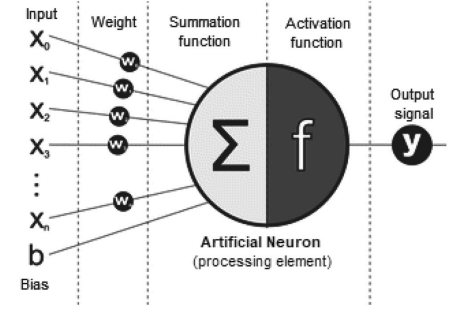
\includegraphics[scale=0.5]{Gambar/ArtificialNeuron.png}
    \caption{Skema Neuron Imitasi} \shortcite{sarker2021deep}
    \label{fig:neuron-scheme}
\end{figure}.

\begin{equation}
    \label{neural}
    y_i(x_i;W_i, b_i) = f(W_i \bullet x_i +b_i)
\end{equation}

Komponen utama jaringan DL terletak pada bagaimana tiap unit neuron saling terkoneksi dalam bentuk \emph{Multi Layer Perceptron} (MLP). Hal ini ditunjukkan pada Gambar \ref{fig:MLP-layers}. Sebuah jaringan MLP tersusun atas satu lapisan input, satu lapisan output, dan sebanyak \(N-2\) lapisan tersembunyi. Lapisan tersembunyi berfungsi sebagai lapisan komputasi yang tersusun atas sejumlah unit neuron dengan fungsi aktivasi untuk memproses data. Kedalaman dari MLP didefinisikan atas banyaknya lapisan tersembunyi sistem untuk mempelajari aspek tertentu dalam data. Akan tetapi, semakin banyak lapisan tersembunyi yang dimiliki model, model MLP dapat menjadi lebih sensitif dan rentan terhadap \emph{overfitting} \shortcite{murtagh1991mlp}.

\begin{figure}[htbp]
    \centering
    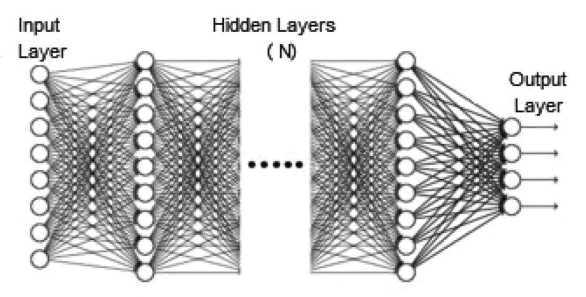
\includegraphics[scale=0.5]{Gambar/MultiLayerPerceptron.png}
    \caption{\emph{Multi Layer Perceptron}} \shortcite{sarker2021deep}
    \label{fig:MLP-layers}
\end{figure}

Konvergensi pemrosesan data jaringan MLP didapatkan melalui proses optimasi bobot dan bias melalui propagasi balik. Metode ini memungkinkan neuron untuk mempelajari karakteristik relevan dalam data dan menghasilkan output yang diharapkan berdasarkan fungsi biaya (\emph{cost function}) model. Fungsi biaya mengatur seberapa besar perbedaan prediksi model dengan target output. Bobot model diperbarui melalui proses minimalisasi nilai fungsi biaya terhadap bobot model secara iteratif \shortcite{shreshta2019AI}.

Proses optimasi bobot MLP dilakukan menggunakan algoritma \emph{gradient descent}. Bobot jaringan neural \(\theta\) diperbarui pada setiap iterasi dengan arah yang berlawanan terhadap gradien dari fungsi biaya, \(\nabla_\theta J(\theta)\). Ukuran besarnya pembaruan bobot dinyatakan oleh laju pembelajaran \(\eta\). Semakin kecil nilai \(\eta\), model belajar lebih lambat, tetapi semakin besar nilai \(\eta\), model rentan mengalami osilasi sehingga tidak mampu mencapai konvergensi \shortcite{ruder2016overview}. Metode \emph{gradient descent} dapat secara matematis dinyatakan dalam persamaan \eqref{grad-descent}. Berbagai metode turunan dari \emph{gradient descent} telah dikembangkan untuk meningkatkan efisiensi proses optimasi, seperti \emph{stochastic gradient descent} (SGD), \emph{adaptive moment-estimation} (ADAM), \emph{Limited-memory Broyden–Fletcher–Goldfarb–Shanno} (L-BFGS), maupun lainnya. 

\begin{equation}
    \label{grad-descent}
    \theta = \theta-\eta \nabla_\theta J(\theta; x^i;y^i)
\end{equation}

Normalisasi data perlu dilakukan selama proses optimasi untuk menjaga stabilitas dan efisiensi penurunan gradien. Normalisasi merupakan proses transformasi data dengan tetap menjaga sifat statistik data. Proses ini mengurangi perbedaan magnitudo fitur sehingga menyeimbangkan distribusi statistik gradien MLP. Dengan demikian, data dalam proses optimasi dapat terstruktur dengan baik tanpa menghambat kinerja model \shortcite{huang2023normalization}.

Pendekatan berbasis data dalam perambatan pulsa serat optik telah ditunjukkan dalam beberapa penelitian. Sebagai contoh, penggunaan jaringan konvolusi (\emph{Convolution Neural Network}/CNN) dalam menangkap perambatan sistem NLS dalam amplifier parametrik serat optik \shortcite{Sui:21}, maupun penggunaan jaringan \emph{Bidirectional Long Short-Term Memory} (Bi-LSTM) untuk memodelkan perambatan pulsa \emph{ultrashort} \shortcite{MARTINS2024103636}. Akan tetapi, metode berbasis data memiliki kelemahan atas dibutuhkannya dataset dalam jumlah besar supaya model dapat melakukan inferensi secara optimal. Selain itu, metode ini juga mengabaikan prinsip fisis yang terdapat pada tiap kasus \shortcite{wang2022applications}.

\section{Physics-Informed Neural Networks}

\emph{Physics-Informed Neural Networks} (PINNs) merupakan jaringan neural terspesialisasi untuk menyelesaikan kasus fisis \shortcite{raissi2019physics}. Hal ini dilakukan melalui modifikasi sistem jejaring neural melalui integrasi persamaan diferensial sistem (\emph{governing equation}) bersama batasan fisis seperti syarat awal dan syarat batas pada fungsi biaya model. Arsitektur PINNs diberikan pada Gambar \ref{Architecture}

\newpage
\begin{figure}[htbp]
    \centering
    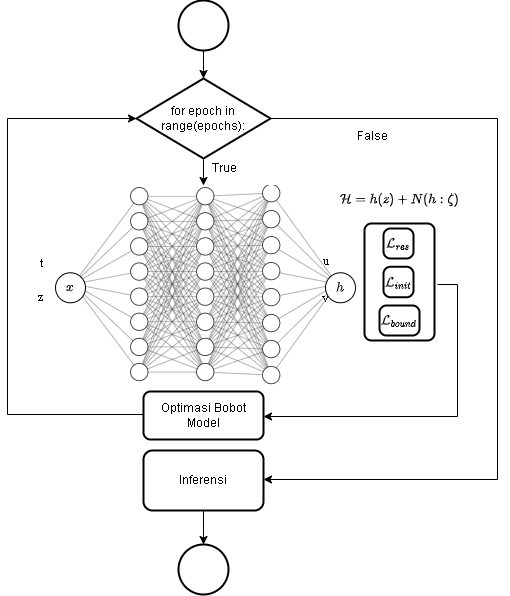
\includegraphics[width=0.6\linewidth]{Gambar/PINN.png}
    \caption{Arsitektur PINNs}
    \label{Architecture}
\end{figure}

Sebuah model PINNs digunakan untuk menyelesaikan sebuah sistem fisis yang diberikan pada persamaan diferensial \(\mathcal{H} = h(x) +N[h: \zeta] = 0\). Model ini menerima titik sampel $x$ sepanjang domain sistem, selanjutnya disebut sebagai titik kolokasi. Lapisan komputasi melakukan perhitungan untuk menghasilkan prediksi solusi persamaan diferensial $h$. Dari perhitungan ini, ditentukan nilai fungsi biaya. Diberikan tiga fungsi biaya pada sistem berupa fungsi biaya residu, $\mathcal{L}_{res}$, fungsi biaya syarat awal $\mathcal{L}_{init}$, dan fungsi biaya syarat batas $\mathcal{L}_{bound}$. Fungsi biaya residu diberikan berdasarkan persamaan diferensial $\mathcal{H}$. Fungsi biaya syarat awal dan fungsi biaya syarat batas didasarkan atas data kondisi awal dan kondisi batas yang diberikan.

\begin{equation}
    \label{residual-loss-func}
    \mathcal{L}_{res} = \frac{1}{N}\sum_{i=1}^N\mathcal{H}^2(x)
\end{equation}

\begin{equation}
    \label{initial-loss-func}
    \mathcal{L}_{init} = \frac{1}{N}\sum_{i=1}^N|h_{init} - \bar{h}_{init}|^2
\end{equation}

\begin{equation}
    \label{boundary-loss-func}
    \mathcal{L}_{init} = \frac{1}{N}\sum_{i=1}^N|h_{bound} - \bar{h}_{bound}|^2
\end{equation}

\noindent
Di mana $\bar{h}$ dan $h$ pada persamaan \eqref{initial-loss-func} dan \eqref{boundary-loss-func} masing-masing menyatakan solusi persamaan yang diketahui dan tebakan solusi persamaan oleh PINNs. Keseluruhan proses ini terus diulangi sehingga mencapai jumlah iterasi (\emph{epochs}) tertentu atau hingga didapatkan hasil yang konvergen. \shortcite{raissi2019physics}. 

Proses Optimasi PINNs dapat dilakukan menggunakan algoritma optimasi ADAM-LBFGS, yaitu perpaduan antara metode optimisasi berbasis \emph{stochastic gradient}, \emph{Adaptive Momentum Estimation} (ADAM) dan pendekatan quasi-Newton, \emph{Limited Memory Broyden–Fletcher–Goldfarb–Shanno} (L-BFGS). Strategi ini umum digunakan guna menawarkan konvergensi yang lebih cepat dan efisiensi komputasi yang tinggi. Performa model umumnya meningkat seiring dengan bertambahnya ukuran sampel dan jumlah epoch pelatihan. Sebaliknya, metode stochastic gradient descent (SGD) murni menghadapi keterbatasan dalam pengelolaan titik kolokasi pada sistem berdimensi tinggi \shortcite{cuomo2022scientific}.

Inisialisasi titik kolokasi model umumnya dilakukan dengan metode \emph{uniform random sampling}, \emph{latin hypercube sampling}, maupun \emph{sobol sequences} \shortcite{pangFPINNN}. Akan tetapi, selama pembelajaran, model mungkin mengalami kesulitan mencapai konvergensi pada daerah tertentu dengan karakteristik fisis yang lebih kompleks \cite{LiuAdapt}. Dengan demikian, pemilihan sampel domain tersebut tidak dapat menyelesaikan masalah ini seorang diri. Maka dari itu, dibutuhkan metode adaptif yang mampu memfokuskan kemampuan komputasi sistem pada daerah yang kesulitan dicapai model. 

\section{Synthetic Minority Over-sampling Technique}

SMOTE (\emph{Synthetic Minority Over-sampling Technique}) merupakan metode yang dirancang untuk mengatasi ketidakseimbangan dataset dalam fungsi klasifikasi. Metode ini bekerja dengan menginterpolasi data sintesis baru antara sebuah titik dan tetangga terdekat, \emph{K-Nearest Neighbor} dalam kelas data minoritas \shortcite{chawla2002smote}. SMOTE telah diaplikasikan dalam berbagai domain dalam fungsi klasifikasi, seperti deteksi penipuan, diagnosis penyakit, maupun pemrosesan sinyal. Kendati metode ini mampu meningkatkan performa klasifikasi, SMOTE berpotensi memberikan distribusi yang menyimpang dari distribusi sebenarnya pada data berdimensi tinggi maupun pada sampel minoritas yang terbatas \shortcite{ELREEDY201932}.
	\addtocontents{toc}{\protect\addvspace{5pt}}
\chapter{METODE PENELITIAN}

\section{Tempat dan Waktu Penelitian}
Penelitian "Optimasi Model \emph{Physics-Informed Neural Networks} untuk Menyelesaikan Persamaan Schrodinger Non-Linear dalam Analisis Perambatan Pulsa Fiber Optik" dilakukan pada Bulan Februari hingga Mei 2025 pada Laboratorium Fisika Komputasi, Jurusan Fisika, Fakultas MIPA, Universitas Brawijaya menggunakan fasilitas AI Center Universitas Brawijaya.

\section{Alat dan Bahan}
Penelitian dilakukan menggunakan \emph{Jupyter Notebook} pada fasilitas \emph{super computer} NVIDIA seri DGX A100 yang disediakan oleh AI Center Universitas Brawijaya. Bahasa pemrograman Python digunakan dengan didukung oleh beberapa pustaka dalam implementasi dan analisis algoritma PINNs. Beberapa pustaka utama yang digunakan meliputi:

\begin{table}[htbp]
    \centering
    \begin{threeparttable}
        \caption{Daftar Pustaka yang Digunakan}
        \begin{tabular}{|p{2cm}|p{8cm}|}
				\hline
				Pustaka & Informasi \\
                \hline 
                \textbf{Pytorch} & Pustaka khusus dalam pembangunan arsitektur akal imitasi PINNs dan optimasi model melalui diferensiasi otomatis.\\
                \hline
                \textbf{Numpy} & Pustaka yang digunakan dalam operasi aljabar linear dan manipulasi array dalam persiapan data.\\
                \hline
                \textbf{Matplotlib} & Pustaka yang digunakan dalam visualisasi perambatan pulsa dan analisis data PINNs.\\
                \hline
                \textbf{Scipy} & Pustaka matematika yang diimplementasikan pada metode SSFM.\\
                \hline
			\end{tabular}
    \end{threeparttable}
\end{table} 

\section{Desain Penelitian}
Penelitian dilakukan dengan pendekatan kuantitatif komputasional untuk mengevaluasi kemampuan generalisasi PINNs dalam menyelesaikan Persamaan Non-Linear Schr\"odinger pada sistem \emph{ultrashort pulse} berdasarkan persamaan \eqref{governing-equation3}.

\begin{align}
    \label{governing-equation3}
    \frac{\partial A(t,z)}{\partial z}
    &+ \frac{\alpha}{2} A(t,z) 
    + i \frac{\beta_2}{2} \frac{\partial^2 A(t,z)}{\partial t^2} \notag \\
    &-  \frac{\beta_3}{6} \frac{\partial^3 A(t,z)}{\partial t^3} 
    - i \gamma |A(t,z)|^2 A(t,z) 
    = 0
\end{align}

Kondisi awal sistem diberikan berdasarkan persamaan secant hiperbolik $A(t,0) = A_0 \frac{1}{\cosh(t/T_0)}$ di mana $A_0$ menyatakan amplitudo pulsa awal dan $T_0$ menyatakan lebar pulsa. Parameter persamaan NLS diberikan pada tabel di bawah:

\begin{table}[htbp]
    \centering
    \begin{threeparttable}
        \caption{Parameter pada Persamaan NLS}
        \label{TabelParam}
        \begin{tabular}{|c|c|}
            \hline
            \textbf{Parameter} & \textbf{Nilai} \\
            \hline
            $\alpha$ & 0.5 dB/m \\
            \hline
            $\beta_2$ & $-5.23 \times 10^{-27}$ s$^2$/m \\
            \hline
            $\beta_3$ & $4.27 \times 10^{-41}$ s$^3$/m \\
            \hline
            $\gamma$ & $18.4 \times 10^{-3}$ W$^{-1}$m$^{-1}$ \\
            \hline
            lebar pulsa ($l$) & $0.58 \times 10^{-12}$ ps \\
            \hline
            amplitudo ($A_0$) & $\sqrt{22.04} \text{W}^{1/2}$ \\
            \hline
            Domain $T$ & $[-1.4 \times 10^{-12},\ 1.4 \times 10^{-12}]$ s \\
            \hline
            Domain $Z$ & $[0,\ 11]$ m \\
            \hline
        \end{tabular}
    \end{threeparttable}
\end{table}

Dalam penelitian ini, selain menyelesaikan persamaan \eqref{governing-equation3} menggunakan model dasar PINNs (selanjutnya disebut sebagai Vanilla-PINNs), turut dirancang modifikasi model PINNs melalui penambahan sampel adaptif. Modifikasi ini diperkenalkan sebagai \emph{SMOTE-Adaptive-Sampling PINNs} (SAS-PINNs). Modifikasi ini mengimplementasikan teknik SMOTE untuk menambahkan titik kolokasi pada daerah yang sulit dipelajari oleh model. Data sampel kolokasi diidentifikasi dan dikelompokkan berdasarkan nilai residu. Sebagian dari data dengan nilai residu tertinggi diperlakukan sebagai kelas minoritas sementara sisanya dianggap sebagai kelas mayoritas. Titik kolokasi pada kelas minoritas kemudian dilakukan \emph{oversampling} menggunakan SMOTE sehingga mencapai target tertentu. Strategi ini dirancang untuk mempermudah konvergensi pada kawasan domain di mana model mengalami kesulitan.

\begin{figure}[htbp]
    \centering
    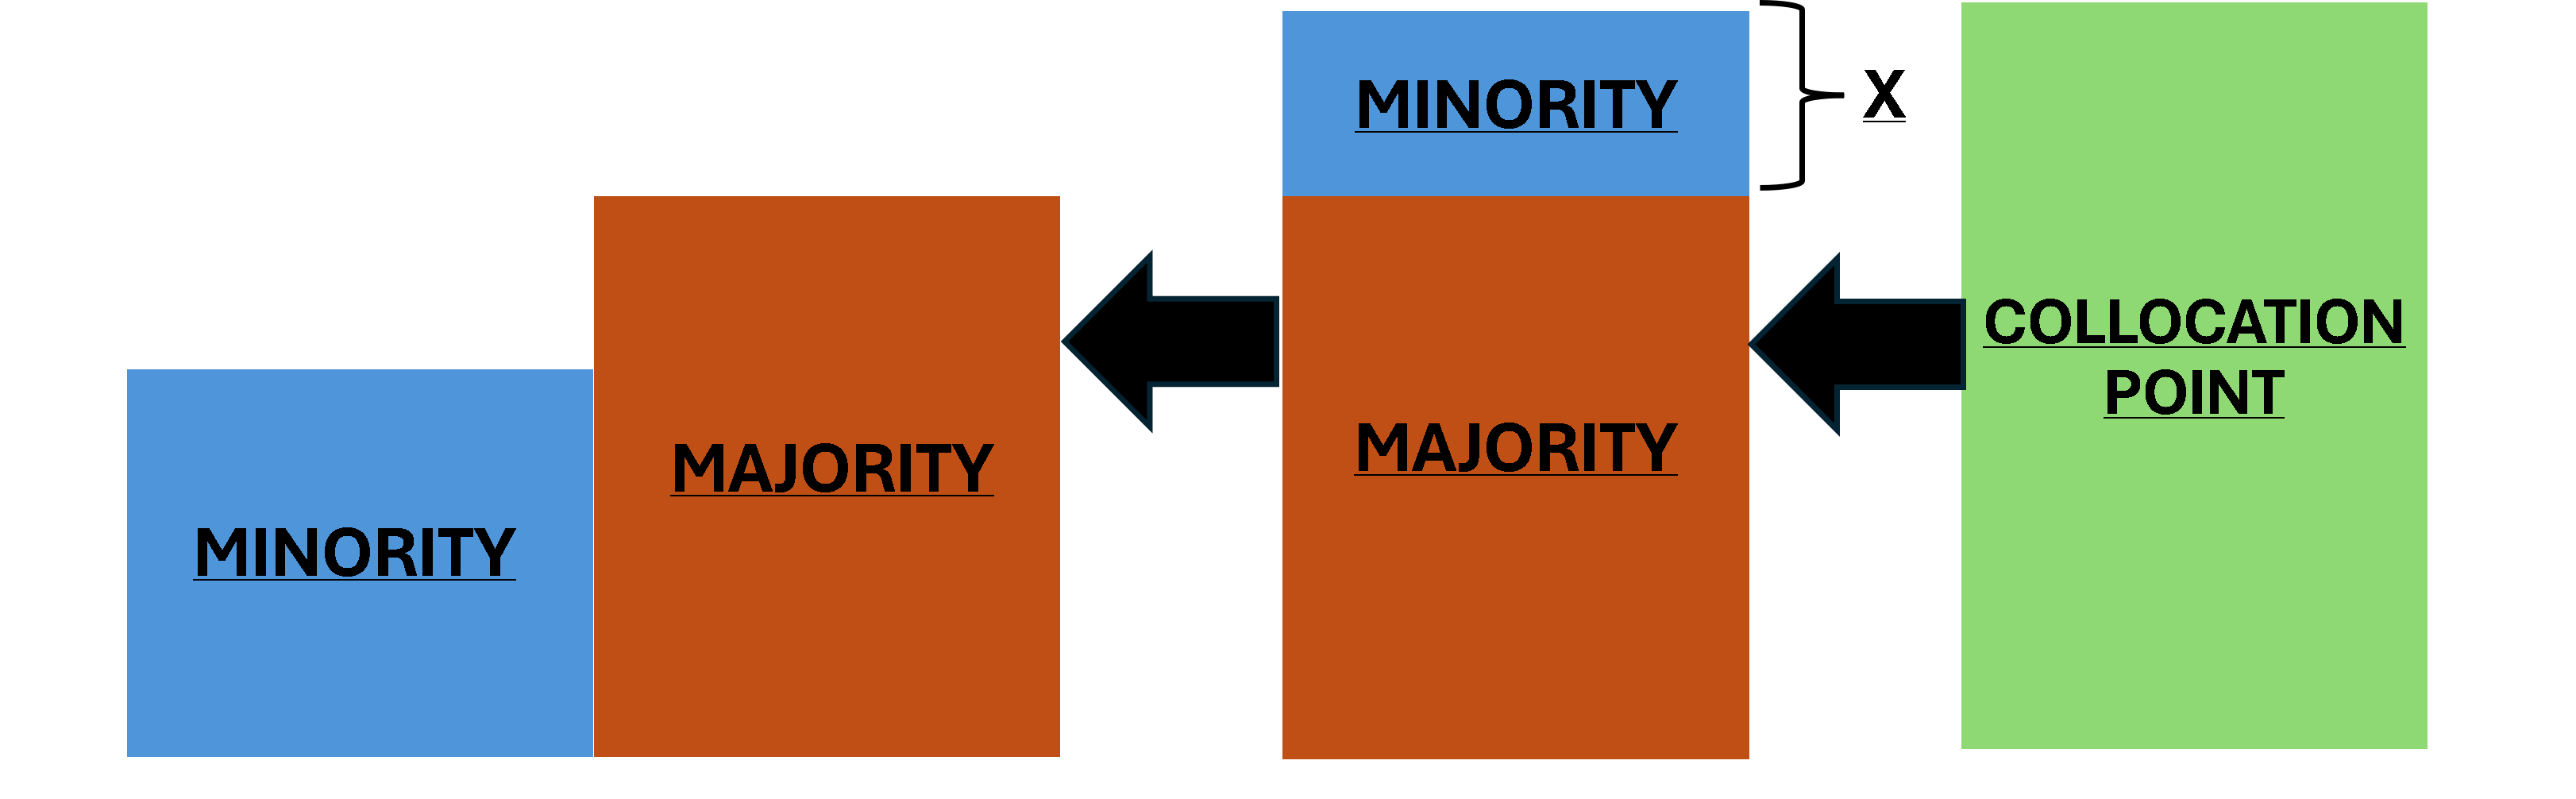
\includegraphics[width=0.8\linewidth]{Gambar/SAS-PINNs-TR.png}
    \caption{Visualisasi Penambahan Sampel SAS-PINNs} 
    \label{fig:SASviz}
\end{figure}

Dalam konfigurasi SAS-PINNs, diperkenalkan dua parameter tambahan berupa Nilai Ambang dan Rasio \emph{Oversampling}. Nilai Ambang menyatakan bagian dari keseluruhan titik kolokasi (dalam desimal) dengan nilai residu tertinggi yang diperlakukan sebagai minoritas. Jumlah nilai ambang tidak dapat melebihi 0.5, atau setengah dari jumlah titik kolokasi. Rasio \emph{oversampling} menyatakan rasio dari jumlah target kelompok minoritas setelah dilakukan penambahan data terhadap kelompok mayoritas.

Evaluasi model dilakukan dengan membandingkan masing-masing model pada tiap perlakuan menggunakan nilai referensi. Nilai referensi ini diperoleh berdasarkan pendekatan numerik SSFM. Parameter evaluasi meliputi akurasi prediksi model terhadap nilai referensi dan kepresisian prediksi model pada beberapa uji ulang. 
\newpage 
\section{Prosedur Penelitian}

Prosedur penelitian diberikan dalam flowchart berikut:

\begin{figure}[htbp]
    \centering
    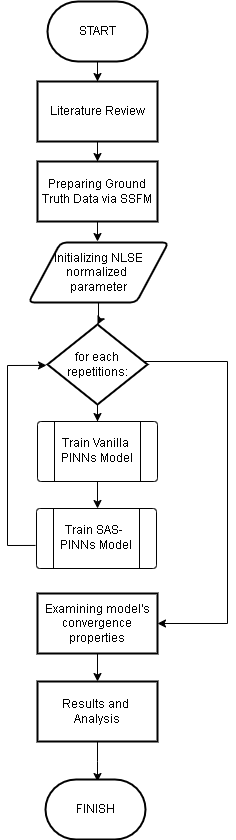
\includegraphics[width=0.32\linewidth]{Gambar/FlowchartFix.png}
    \caption{Flowchart Penelitian} 
    \label{fig:main-flowchart}
\end{figure}

\newpage
Peninjauan pustaka dilakukan untuk mendapatkan informasi terkait yang diperlukan dalam penelitian. Selanjutnya, data referensi disintesis atas validasi prediksi PINNs menggunakan SSFM. Parameter ternormalisasi kemudian diinisialisasi sebelum proses pembelajaran PINNs dilakukan. Pembelajaran dilakukan menggunakan struktur jaringan neural Vanilla-PINNs dan SAS-PINNs. Sifat konvergensi model dianalisis dan dibandingkan satu sama lain berdasarkan nilai error model dan presisi pada beberapa uji ulang. 


\subsection{Sintesis Data Referensi Melalui SSFM}
Data referensi diperlukan sebagai validasi atas prediksi PINNs. Data ini disusun menggunakan SSFM sebagai metode yang umum digunakan dalam menyelesaikan persamaan NLS. Grid numerik SSFM diinisialisasi sebagai \(2^{11}\) \emph{timesteps} dan \(2^7\) \emph{lengthsteps}. Dengan demikian, dinamika propagasi pulsa memiliki resolusi yang cukup tinggi untuk dibandingkan dengan model PINNs. Flowchart dari SSFM diberikan pada Gambar \ref{fig:ssfm-flowchart}.

Operator nonlinear $\mathcal{N}$ dan linear $\mathcal{L}$ diberikan dalam persamaan \eqref{nonlinear3} dan \eqref{linear3}

\begin{equation}
    \hat{\mathcal{N}} = i\gamma dz
    \label{nonlinear3}
\end{equation}

\begin{equation}
    \hat{\mathcal{L}} = \exp\left( i\frac{\beta_2}{2\omega^2}-i\frac{\beta_3}{6\omega^3} -\alpha/2 \right)dz
    \label{linear3}
\end{equation}

Penyelesaian operator nonlinear dan linear diberikan dalam persamaan \eqref{nonlinear-step} dan \eqref{linear-step} sebagai: 

\begin{equation}
    A_N(t,z+dz) = A(t,z)\exp(\hat{\mathcal{N}}|A|^2)
    \label{nonlinear-step}
\end{equation}

\begin{equation}
    A(t,z+dz) = \mathcal{F}^{-1}(\mathcal{F}(A_N)\hat{\mathcal{L}})
    \label{linear-step}
\end{equation}

\newpage
\begin{figure}[htbp]
    \centering
    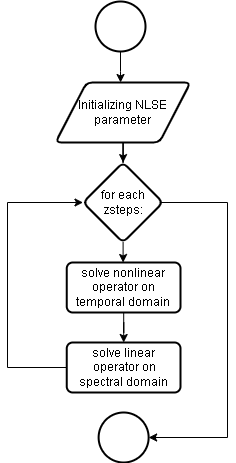
\includegraphics[width=0.4\linewidth]{Gambar/SSFM-F.png}
    \caption{Flowchart SSFM} 
    \label{fig:ssfm-flowchart}
\end{figure}


\subsection{Inisialisasi Parameter Persamaan NLS dalam PINNs}

Persamaan NLS didasarkan atas parameter Tabel \ref{TabelParam}. Nilai \(\alpha\) pada satuan dB perlu dikonversi ke Nepers dengan dikalikan \(\dfrac{\log(10)}{10}\). Selain itu normalisasi  perlu dilakukan pada fungsi \eqref{governing-equation3} dikarenakan skala nilai parameter yang terpaut jauh. Perbedaan ini berpotensi menyebabkan ketidakseimbangan pembelajaran PINNs. Normalisasi persamaan dilakukan dengan mengubah variabel $(t,z)$ menjadi unit satuan sebagai $(t,z) = (T\hat{t}, Z\hat{z})$ untuk meningkatkan stabilitas numerik dan mempercepat konvergensi pembelajaran. Maka dari itu, domain perambatan pulsa diatur sebagai $\hat{t} \in [-1,1]$ dan $\hat{z} \in [0,1]$. Persamaan diferensial ternormalisasi, dengan demikian, menjadi:

\begin{align}
    \mathcal{H} =\frac{\partial A(\hat{t},\hat{z})}{\partial \hat{z}}
    &+ \frac{\alpha Z}{2} A(\hat{t},\hat{z}) 
    + i \frac{\beta_2 Z}{2T^2} \frac{\partial^2 A(\hat{t},\hat{z})}{\partial \hat{t}^2} \notag \\
    &-  \frac{\beta_3 Z}{6T^3} \frac{\partial^3 A(\hat{t},\hat{z})}{\partial \hat{t}^3} 
    - i \gamma Z |A(\hat{t},\hat{z})|^2 A(\hat{t},\hat{z})
    \label{normalized-eq}
\end{align}
\subsection{Inisialisasi Model PINNs}

Model PINNs diinisialisasi sebagai jaringan neural dengan dua input (\(t,x\)), dua neuron output (\(u,v\)), dan empat lapisan tersembunyi, masing-masing berisi 128 neuron. Dua neuron input difungsikan untuk menerima dimensi temporal dan spasial model. Sementara itu, dua neuron output, masing-masing merepresentasikan bagian riil dan imajiner dari solusi persamaan. Setiap lapisan tersembunyi dilengkapi dengan fungsi aktivasi \(\tanh()\). 

Fungsi biaya PINNs tersusun oleh fungsi biaya residu dan fungsi biaya data berdasarkan prediksi kondisi awal dan syarat batas Dirichlet serta Neumann. Masing-masing fungsi biaya diberikan faktor pembobot untuk mengatur kontribusi dari masing-masing komponen. Bobot komponen untuk fungsi residual diatur dan syarat batas diatur sebagai 1, sementara fungsi biaya kondisi awal sebagai 10 oleh karena sensitivitas PINNs terhadap kondisi awal.

\begin{equation}
    \mathcal{L}_{total} = \lambda_{i}\mathcal{L}_{init}+\lambda_{r}\mathcal{L}_{residue}+\lambda_{b}\mathcal{L}_{bound}
    \label{total-loss}
\end{equation}

\noindent
Fungsi biaya residual $\mathcal{L}_{residue}$ diberikan sebagai: 

\begin{equation}
    \mathcal{L}_{residue} =  \sum_{d_i = 1}^{N_{\mathcal{H}}} \mathcal{H}_u^2+\mathcal{H}_v^2
\end{equation}

\noindent
Sementara itu, fungsi biaya syarat awal dinyatakan dengan: 

\begin{equation}
    \mathcal{L}_{init} =  \sum_{d_i = 1}^{N_{\mathcal{I}}} \bigg( (u_{init}-\bar{u}_{init})^2 + (v_{init}-\bar{v}_{init})^2 \bigg)
\end{equation}

\noindent 
dengan \(\bar{u}_{init}\) dan \(\bar{v}_{init}\) menyatakan pulsa riil dan imajiner yang diketahui.

\noindent
Syarat batas Dirichlet dan Neumann periodik diberikan pada persamaan. Syarat ini menyatakan simetri pada kedua ujung domain, $A(-1,z) = A(1,z)$ dan $$\frac{\partial}{\partial t}(-1,z) = \frac{\partial}{\partial t}A(1,z)$$

\begin{equation}
    \mathcal{L}_{boundD} =  \frac{1}{N_B}\sum_{d_i = 1}^{N_B} \left((u(1,z)-u(-1,z)^2 + (v(1,z)-v(-1,z))^2 \right)
\end{equation}

\begin{align}
\mathcal{L}_{boundN} 
&= \frac{1}{N_B} \sum_{d_i = 1}^{N_B} \Bigg[
    \left( \left.\frac{\partial u}{\partial t} \right|_{t = -1} - 
           \left.\frac{\partial u}{\partial t} \right|_{t = 1} \right)^2 
    \notag \\ &\quad
    + \left( \left.\frac{\partial v}{\partial t} \right|_{t =-1} - 
             \left.\frac{\partial v}{\partial t} \right|_{t = 1} \right)^2
\Bigg]
\end{align}

\begin{equation}
     \mathcal{L}_{bound} = \mathcal{L}_{boundN} + \mathcal{L}_{boundD}
\end{equation}

Model dioptimasi menggunakan strategi optimasi gabungan: ADAM selama 40000 epoch dan LBFGS selama 5000 epoch. Laju pembelajaran ADAM diatur sebesar \(10^{-4}\) dan berkurang sebanyak 10\% untuk tiap 5000 epoch. Pendekatan ini menggabungkan keunggulan dari kedua metode, dengan ADAM memberikan laju konvergensi yang cepat, sementara LBFGS memberikan presisi lebih tinggi pada tahap akhir pelatihan

\newpage
\subsection{Pembelajaran PINNs}

Pembelajaran PINNs terbagi atas tahapan pembelajaran Vanilla-PINNs dan SAS-PINNs dengan algoritma yang diberikan pada flowchart di bawah

\begin{figure}[htbp]
    \centering
    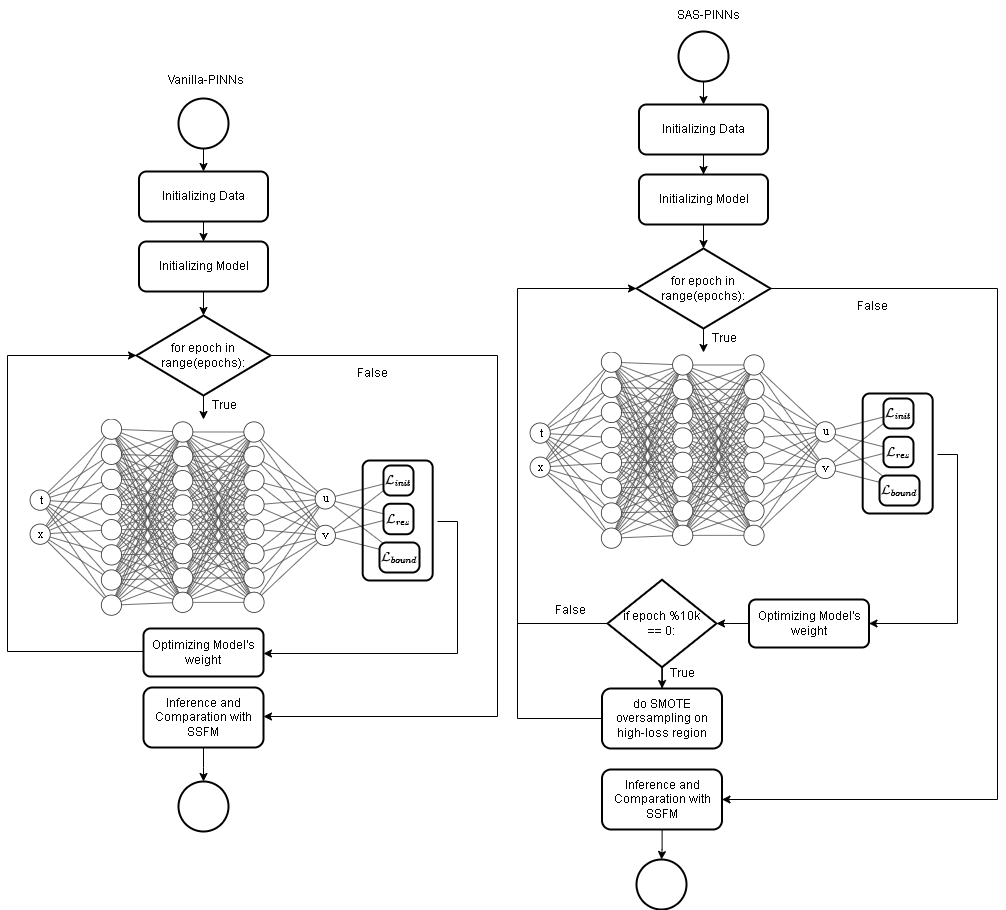
\includegraphics[width=1\linewidth]{Gambar/PINN-Diagram.png}
    \caption{Flowchart PINNs}
    (a) (kiri) Vanilla-PINNs; (b) (kanan) SAS-PINNs
    \label{fig:enter-label}
\end{figure}

Data yang diperlukan PINNs disampel menggunakan metode \emph{Latin Hypercube Sampling}. Jumlah sampel titik awal diberikan sebagai 500 dan titik batas sebagai 500 pada kedua sisi. Pada Vanilla-PINNs, jumlah titik kolokasi menjadi variabel bebas yang divariasikan pada [2.000, 5.000, 10.000, 20.000, dan 40.000]. Hal ini dilakukan untuk menilai bagaimana pengaruh jumlah sampel domain terhadap konvergensi PINNs. Proses pembelajaran PINNs pada tiap variasi jumlah sampel diulangi pada \emph{random seed} [0, 25, 420, 9999] untuk mendapatkan hasil yang lebih akurat. 

Pembelajaran SAS-PINNs dilakukan dengan jumlah sampel titik awal dan titik batas, serta struktur model dan strategi optimasi yang sama dengan model sebelumnya. Akan tetapi, jumlah titik kolokasi diatur tetap sejumlah 10.000. Konfigurasi nilai ambang dan rasio \emph{oversampling} ialah: 

\begin{table}[htbp]
    \centering
    \begin{threeparttable}
        \caption{Nilai Ambang dan Rasio SAS-PINNs}
        \begin{tabular}{|p{5cm}|p{4cm}|}
				\hline
				Nilai Ambang & Rasio \\
                \hline 
                0.45 & 1\\
                \hline
                0.35 & 0.7 \\
                \hline
                0.25 & 0.4 \\
                \hline
                0.15 & 0.25 \\
                \hline
			\end{tabular}
    \end{threeparttable}
\end{table} 

Pemilihan kedua parameter ini didasarkan atas jumlah data yang ditambahkan dan bagaimana data tersebut terdistribusi. Semakin kecil nilai ambang, data augmentasi SAS-PINNs semakin terfokus pada daerah dengan residu tertinggi. Namun, nilai ambang yang lebih besar mengakibatkan distribusi data yang lebih tersebar. Masing-masing konfigurasi SAS-PINNs dilakukan perulangan dengan empat \emph{random seed} yang sama dengan percobaan Vanilla-PINNs. Proses augmentasi titik kolokasi dilakukan untuk setiap 10000 \emph{epoch} dalam strategi optimasi ADAM. 


\subsection{Evaluasi Model}
Model dievaluasi berdasarkan akurasinya terhadap nilai referensi SSFM dan konsistensi prediksi model pada beberapa uji ulang untuk \emph{random seed yang berbeda}. Akurasi model diukur menggunakan metrik \emph{mean square error} (MSE). Presisi model diukur dengan mengamati persebaran nilai MSE dan rata-rata MSE model pada masing-masing perlakuan. 


\begin{equation}
    MSE = \frac{1}{N}\sum_{i=1}^N |A_i-\bar{A}_i|^2
\end{equation}

\noindent
nilai $A$ menyatakan prediksi pulsa kompleks PINNs, sementara $\bar{A}$ menyatakan pulsa referensi. 



	\addtocontents{toc}{\protect\addvspace{5pt}}
\chapter{HASIL DAN PEMBAHASAN}

\section{Analisis Data Referensi SSFM}

Data referensi perambatan pulsa diperoleh melalui teknik numerik SSFM. Gambar \ref{fig:reference} menunjukkan adanya peningkatan daya maksimum pulsa diiringi oleh proses kompresi terhadap kondisi awal. Keseluruhan proses perambatan pulsa dipengaruhi oleh nilai dispersi kecepatan grup $\beta_2$ dan interaksinya terhadap nonlinearitas serat optik $\gamma$.


\begin{figure}[htbp]
    \centering
    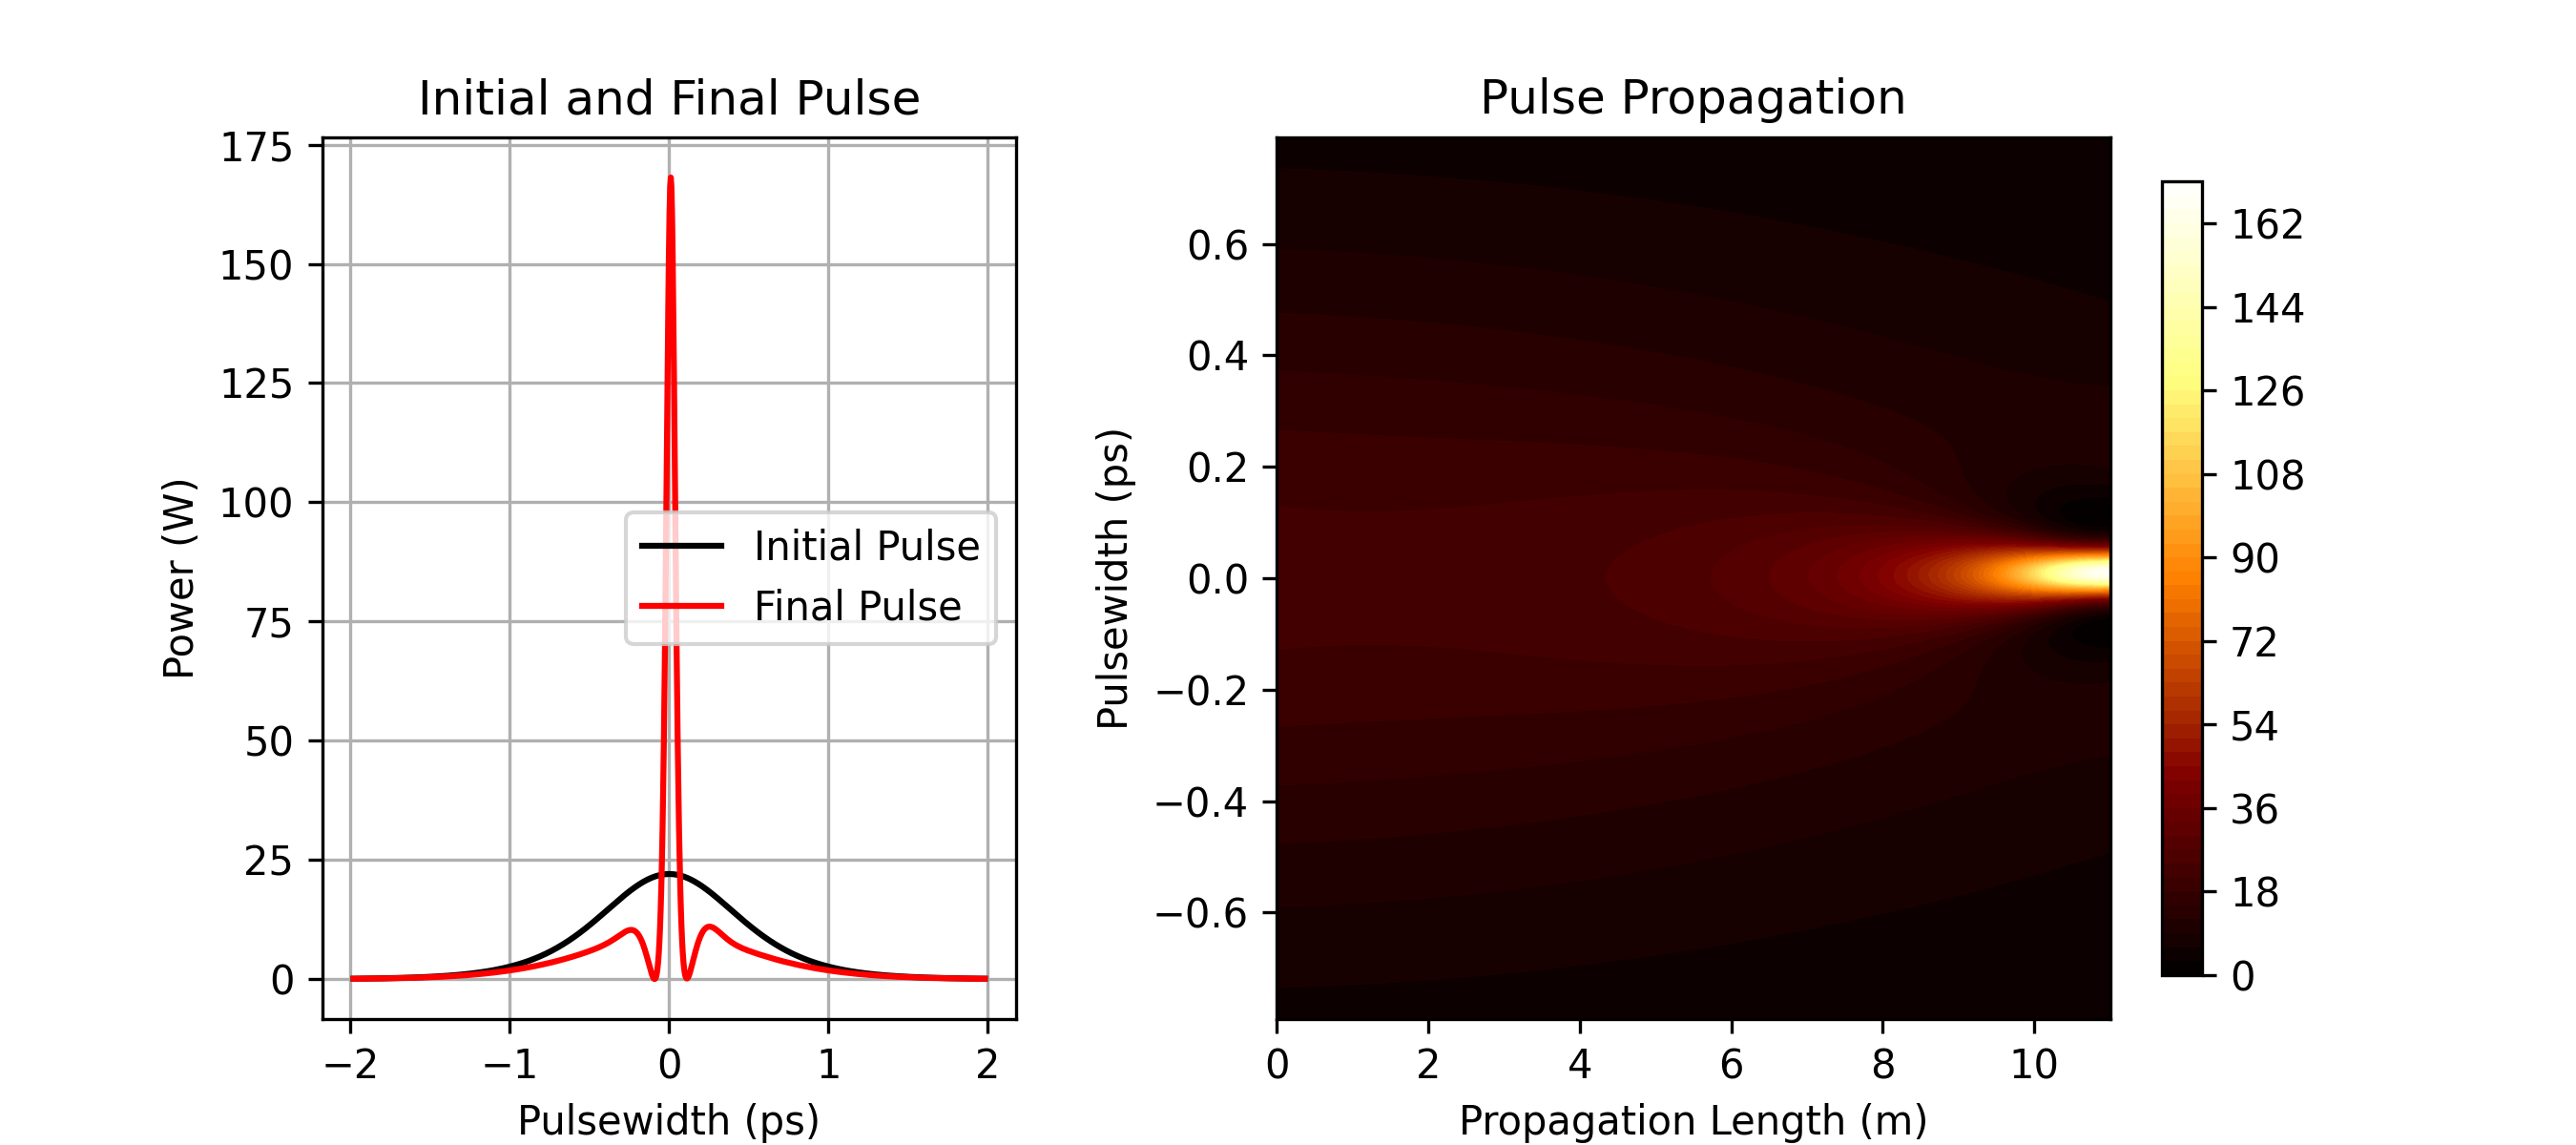
\includegraphics[width=1\linewidth]{Gambar/GroundTruth3D.png}
    \caption{Daya Pulsa Referensi (SSFM)}
    (a) Kondisi Awal dan Akhir; (b) Perambatan Pulsa
    \label{fig:reference}
\end{figure}

Nilai $\beta_2$ negatif menunjukkan sistem dispersi anomali di mana gelombang berfrekuensi tinggi bergerak lebih cepat. Hal ini menyebabkan terjadinya kompresi pulsa ketika efek dispersi mampu mengimbangi nonlinearitas serat optik. Sementara itu, orde dispersi ketiga $\beta_3$ menyatakan perubahan nilai dispersi kecepatan grup yang tidak dapat diabaikan pada sistem dengan lebar pulsa yang sangat pendek $T_0 < 1 \textbf{ ps}$.

\begin{figure}[htbp]
    \centering
    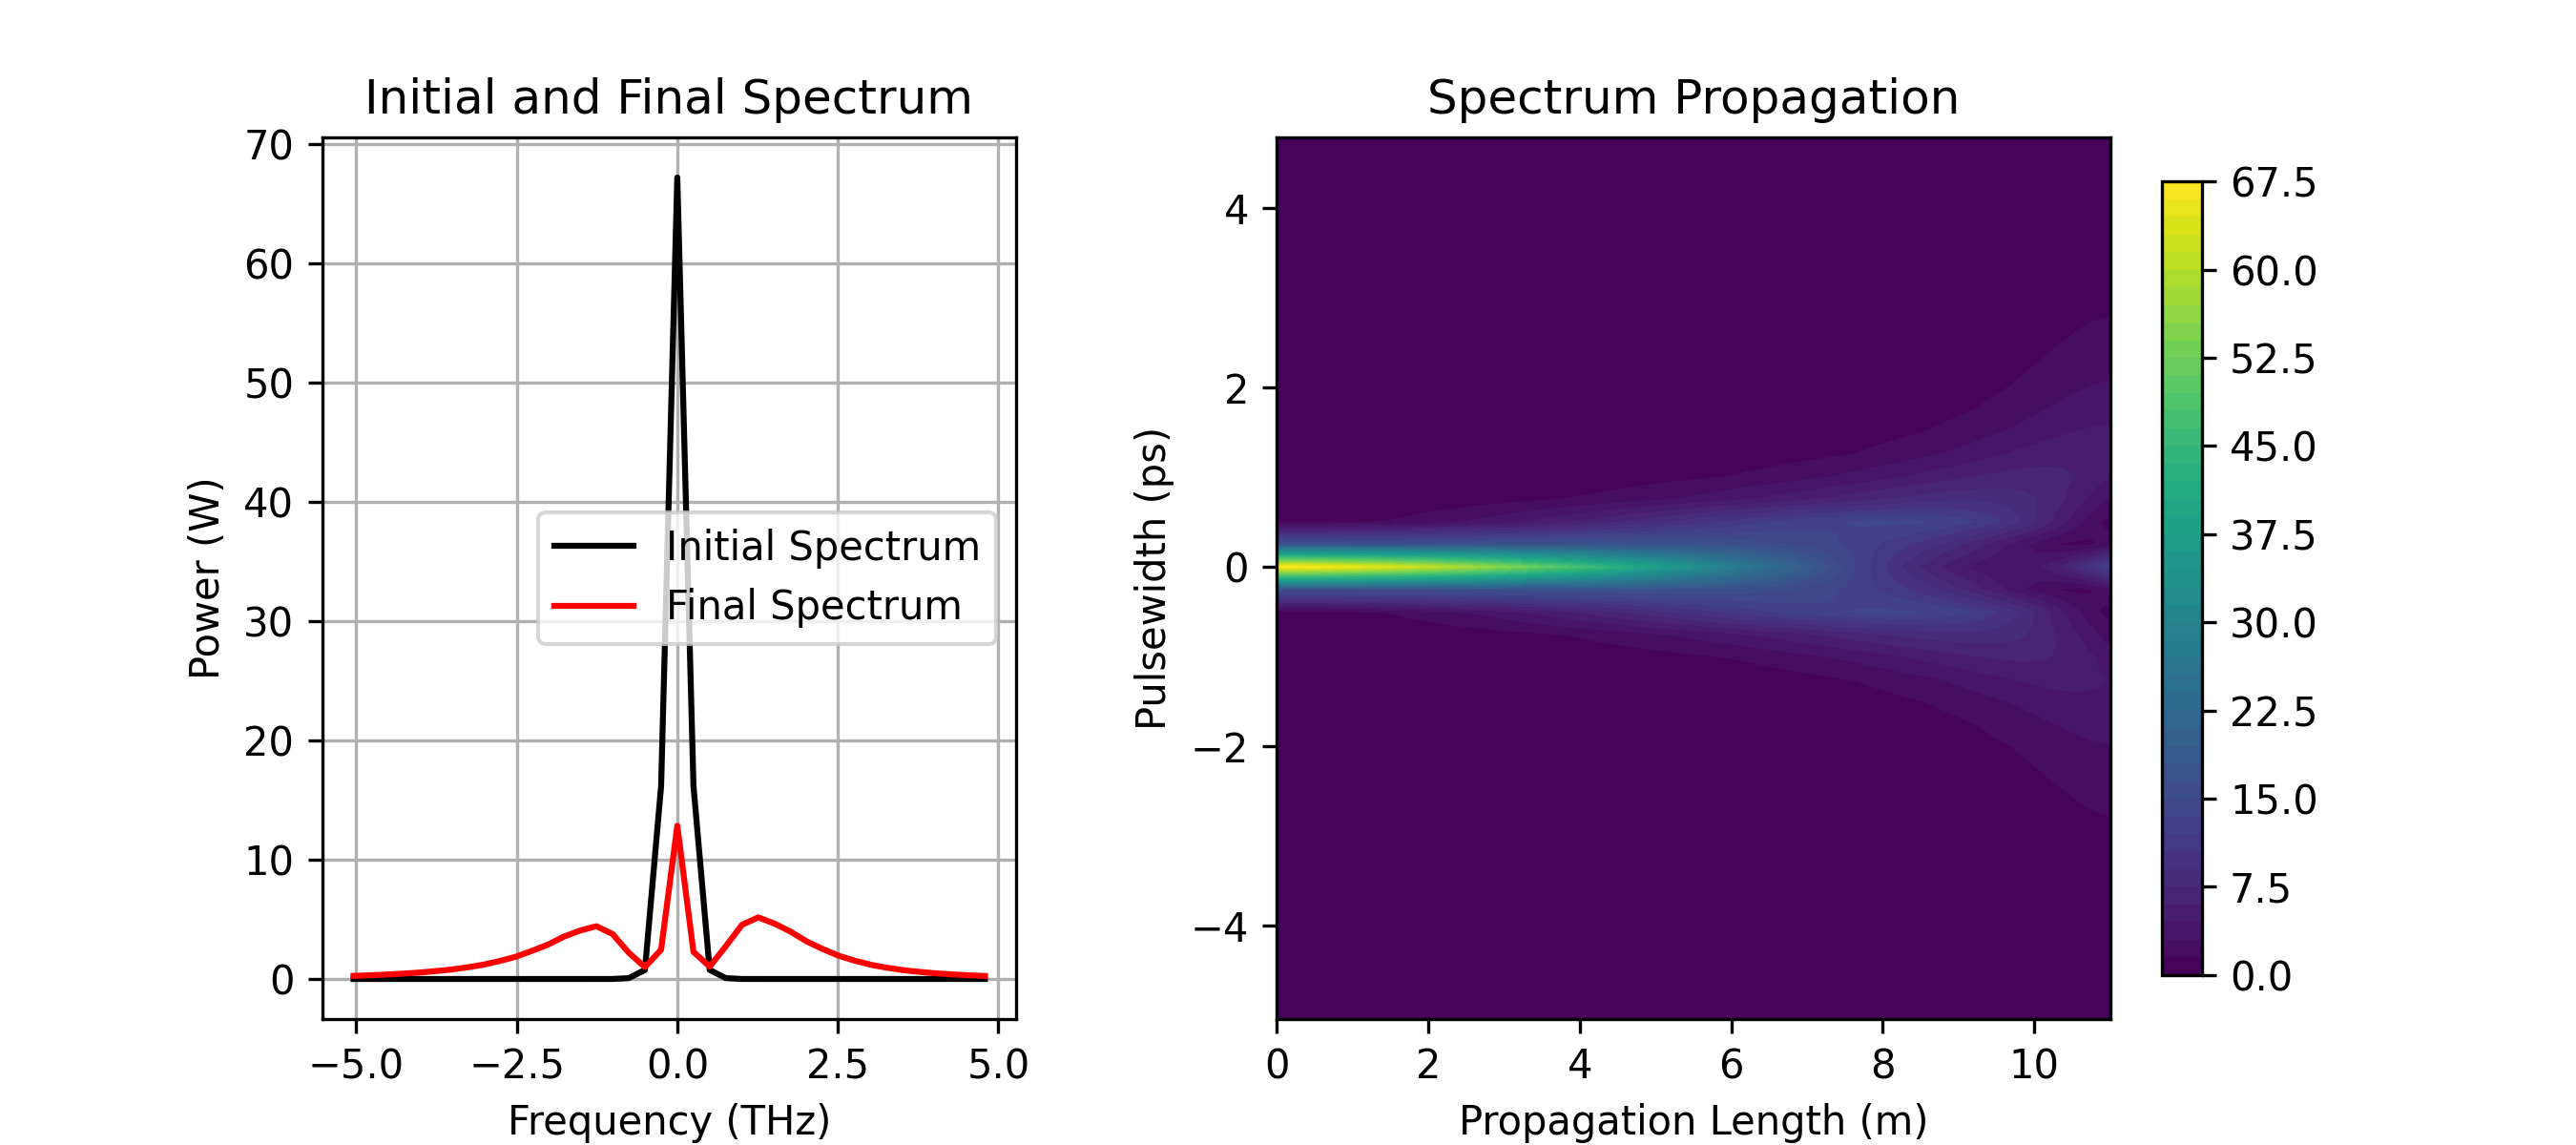
\includegraphics[width=1\linewidth]{Gambar/GroundTruthS3D.png}
    \caption{Spektrum Ground Truth (SSFM)}
    (a) Kondisi Awal dan Akhir; (b) Perambatan Spektrum
    \label{fig:referenceS}
\end{figure}

Distribusi intensitas pulsa pada domain frekuensi ditunjukkan dalam Gambar \ref{fig:referenceS}, di mana pulsa mengalami pelebaran spektrum frekuensi. Hal ini disebabkan oleh modulasi fase tunggal dalam serat optik. Indeks bias nonlinear serat menyebabkan dihasilkannya fase tambahan seiring perambatan pulsa. Frekuensi pulsa kemudian bergeser menjadi lebih tinggi, menghasilkan spektrum yang lebih lebar. Namun, oleh karena gelombang dengan frekuensi lebih tinggi bergerak lebih cepat, komponen gelombang ini menyebabkan durasi pulsa menjadi lebih pendek sehingga pulsa terkompresi.

\section{Evaluasi Hasil Prediksi Vanilla-PINNs}
Hasil inferensi model Vanilla-PINNs menunjukkan karakteristik yang berbeda-beda pada tiap titik kolokasi. Gambar \ref{fig:pulsePINNs} menunjukkan perbandingan antara data pulsa referensi dan data pulsa prediksi model beserta distribusi nilai error dari tiga sampel model. Prediksi PINNs dibandingkan dengan data referensi SSFM, yang ditunjukkan pada \ref{fig:pulsePINNs} (a), melalui \emph{mean square error} (MSE).

\newpage
\begin{figure}[htbp]
    \centering
    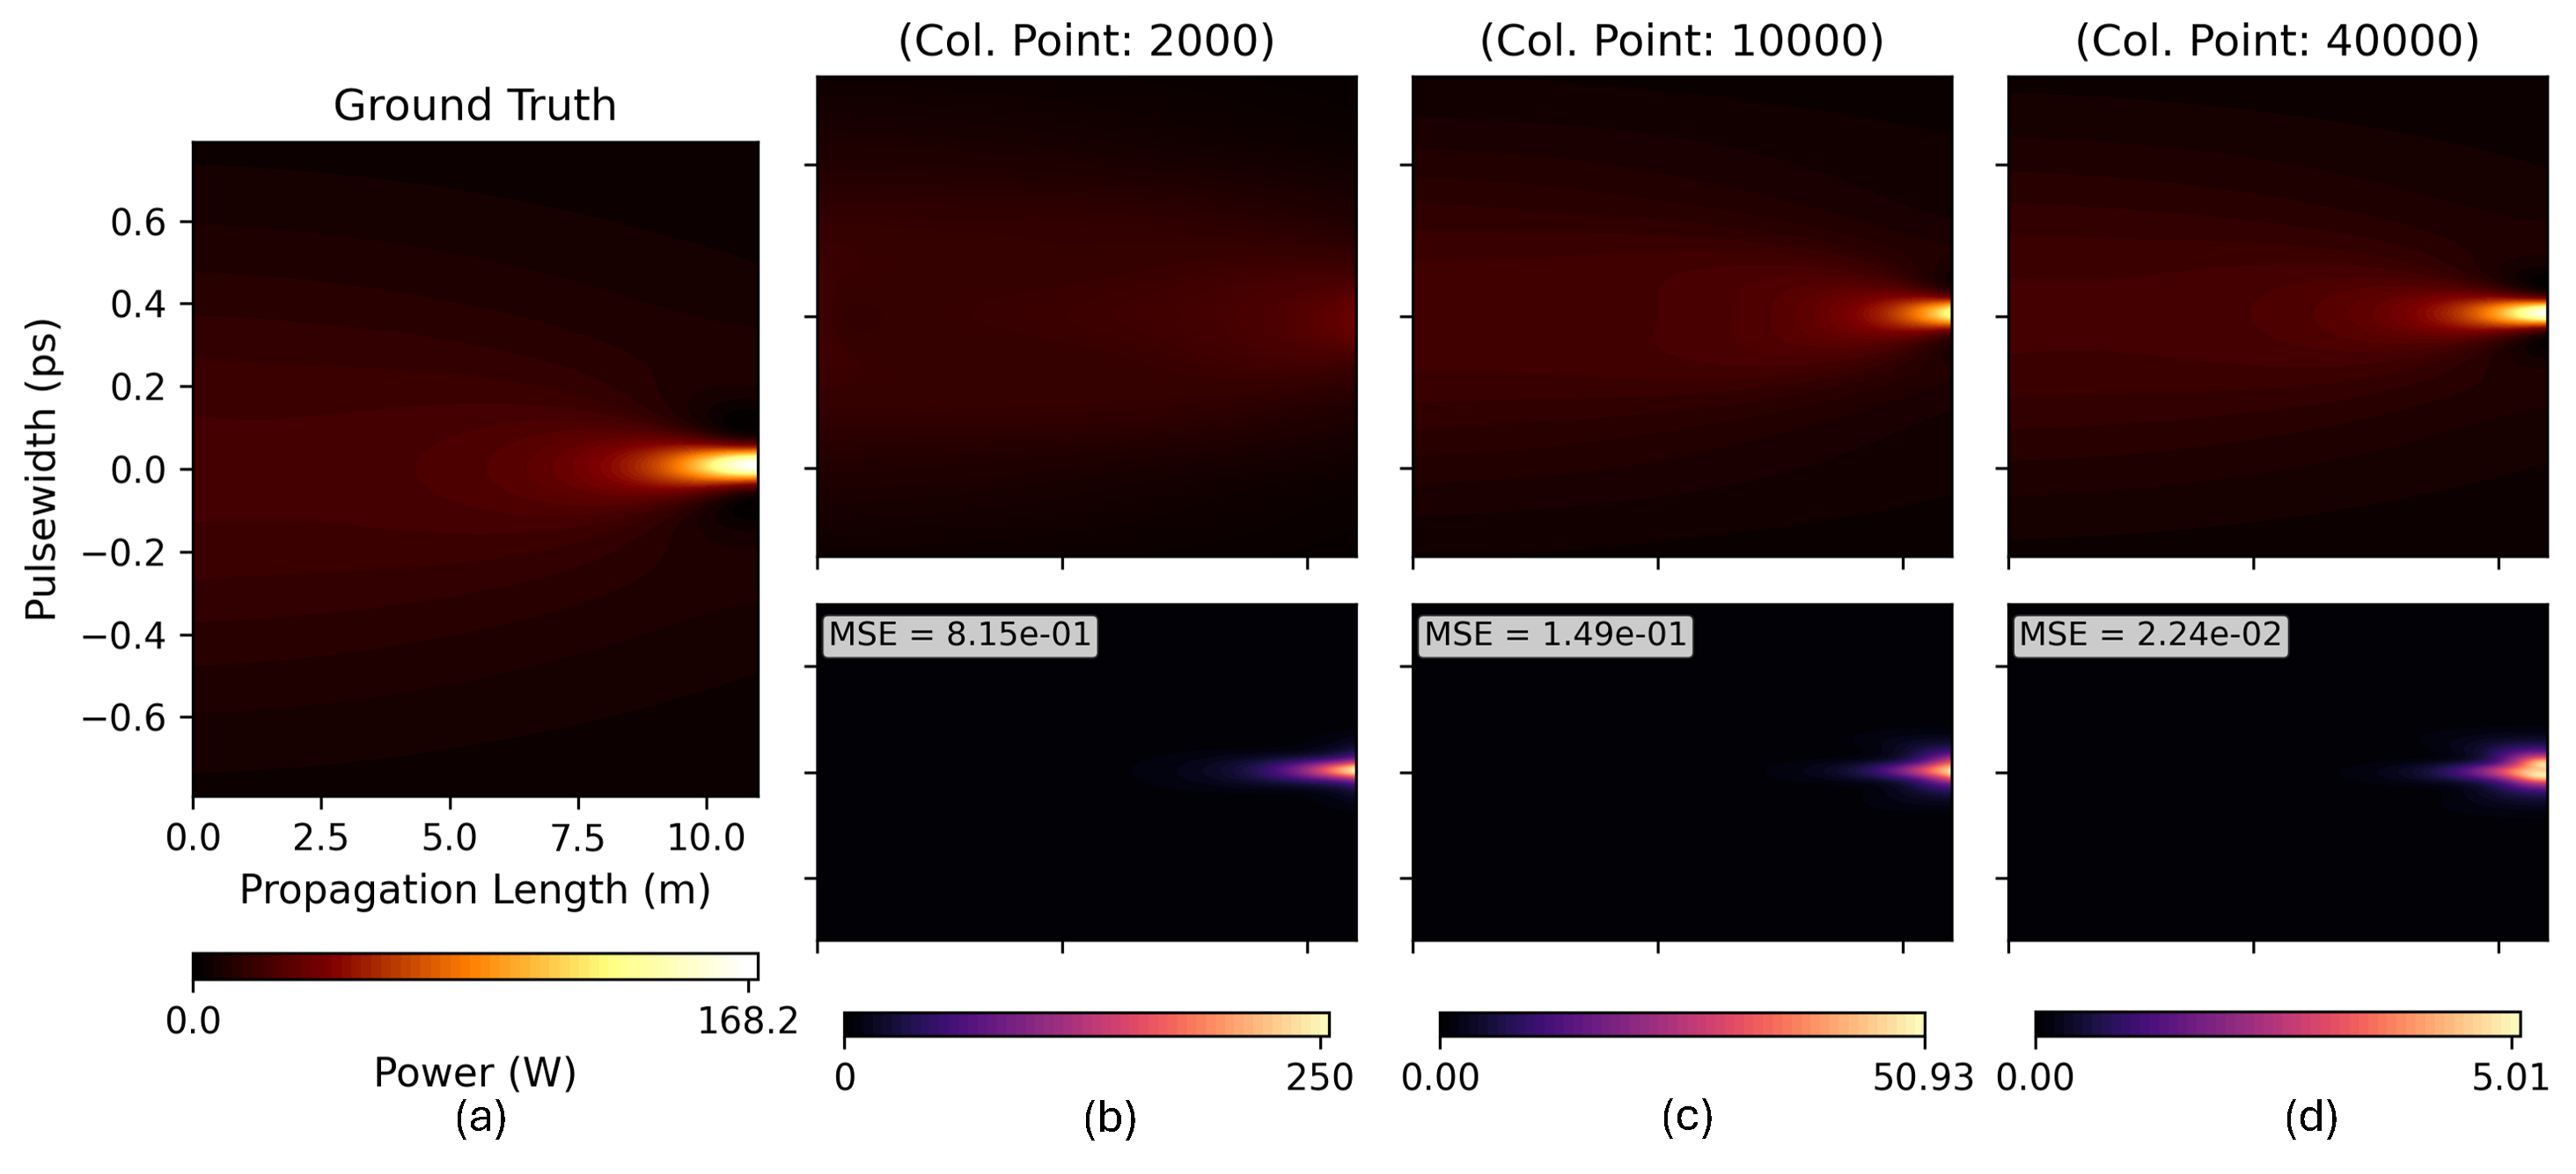
\includegraphics[width=0.9\linewidth]{Gambar/resultsVanilla.png}
    \caption{Distribusi daya pulsa (PINNs)}
    (a) Referensi Numerik, (b)--(d) Prediksi PINNs dengan Titik Kolokasi 2.000, 5.000, dan 10.000 (atas: daya pulsa; bawah: error prediksi (MSE))
    \label{fig:pulsePINNs}
\end{figure}

Ketiga model menunjukkan kesulitan dalam memprediksi proses kompresi pulsa pada jarak 10--11 meter, diberikan pada distribusi error Gambar \ref{fig:pulsePINNs} (b)--(d) bagian bawah. Akan tetapi, ketiga model memiliki nilai MSE yang berbeda. Model dengan 2.000 titik kolokasi tidak mampu menangkap karakteristik penguatan pulsa dengan nilai MSE 0.815. Selain itu, terdapat peningkatan pada model dengan 10.000 titik kolokasi dengan MSE 0.149. Hasil terbaik diperoleh pada model dengan 40.000 titik kolokasi yang mampu dengan baik menangkap proses perambatan pulsa dengan MSE $2.204\times10^{-2}$.

Gambar \ref{fig:specPINNs} menunjukkan bagaimana transformasi prediksi model PINNs pada domain spektral. Kesulitan model dalam memodelkan penguatan pulsa menyebabkan nilai error yang terfokus pada proses pelebaran spektrum pada jarak 10--11 meter. Sama halnya dengan Gambar \ref{fig:pulsePINNs}, dibandingkan dengan referensi numerik pada \ref{fig:specPINNs} (a), model dengan 2.000 sampel domain tidak mampu menangkap pergeseran spektrum dengan benar, sementara hasil terbaik turut diperoleh pada model dengan 40.000 sampel. Akan tetapi, nilai MSE domain spektral memberikan hasil yang lebih kecil dari domain temporal. Hal ini dapat dijelaskan dengan nilai daya spektrum yang lebih kecil dan tersebar dibanding daya pulsa yang lebih besar dan terfokus pada titik kompresi. Oleh karena itu, akumulasi error dari daya temporal lebih besar dari daya spektrum.

\begin{figure}[htbp]
    \centering
    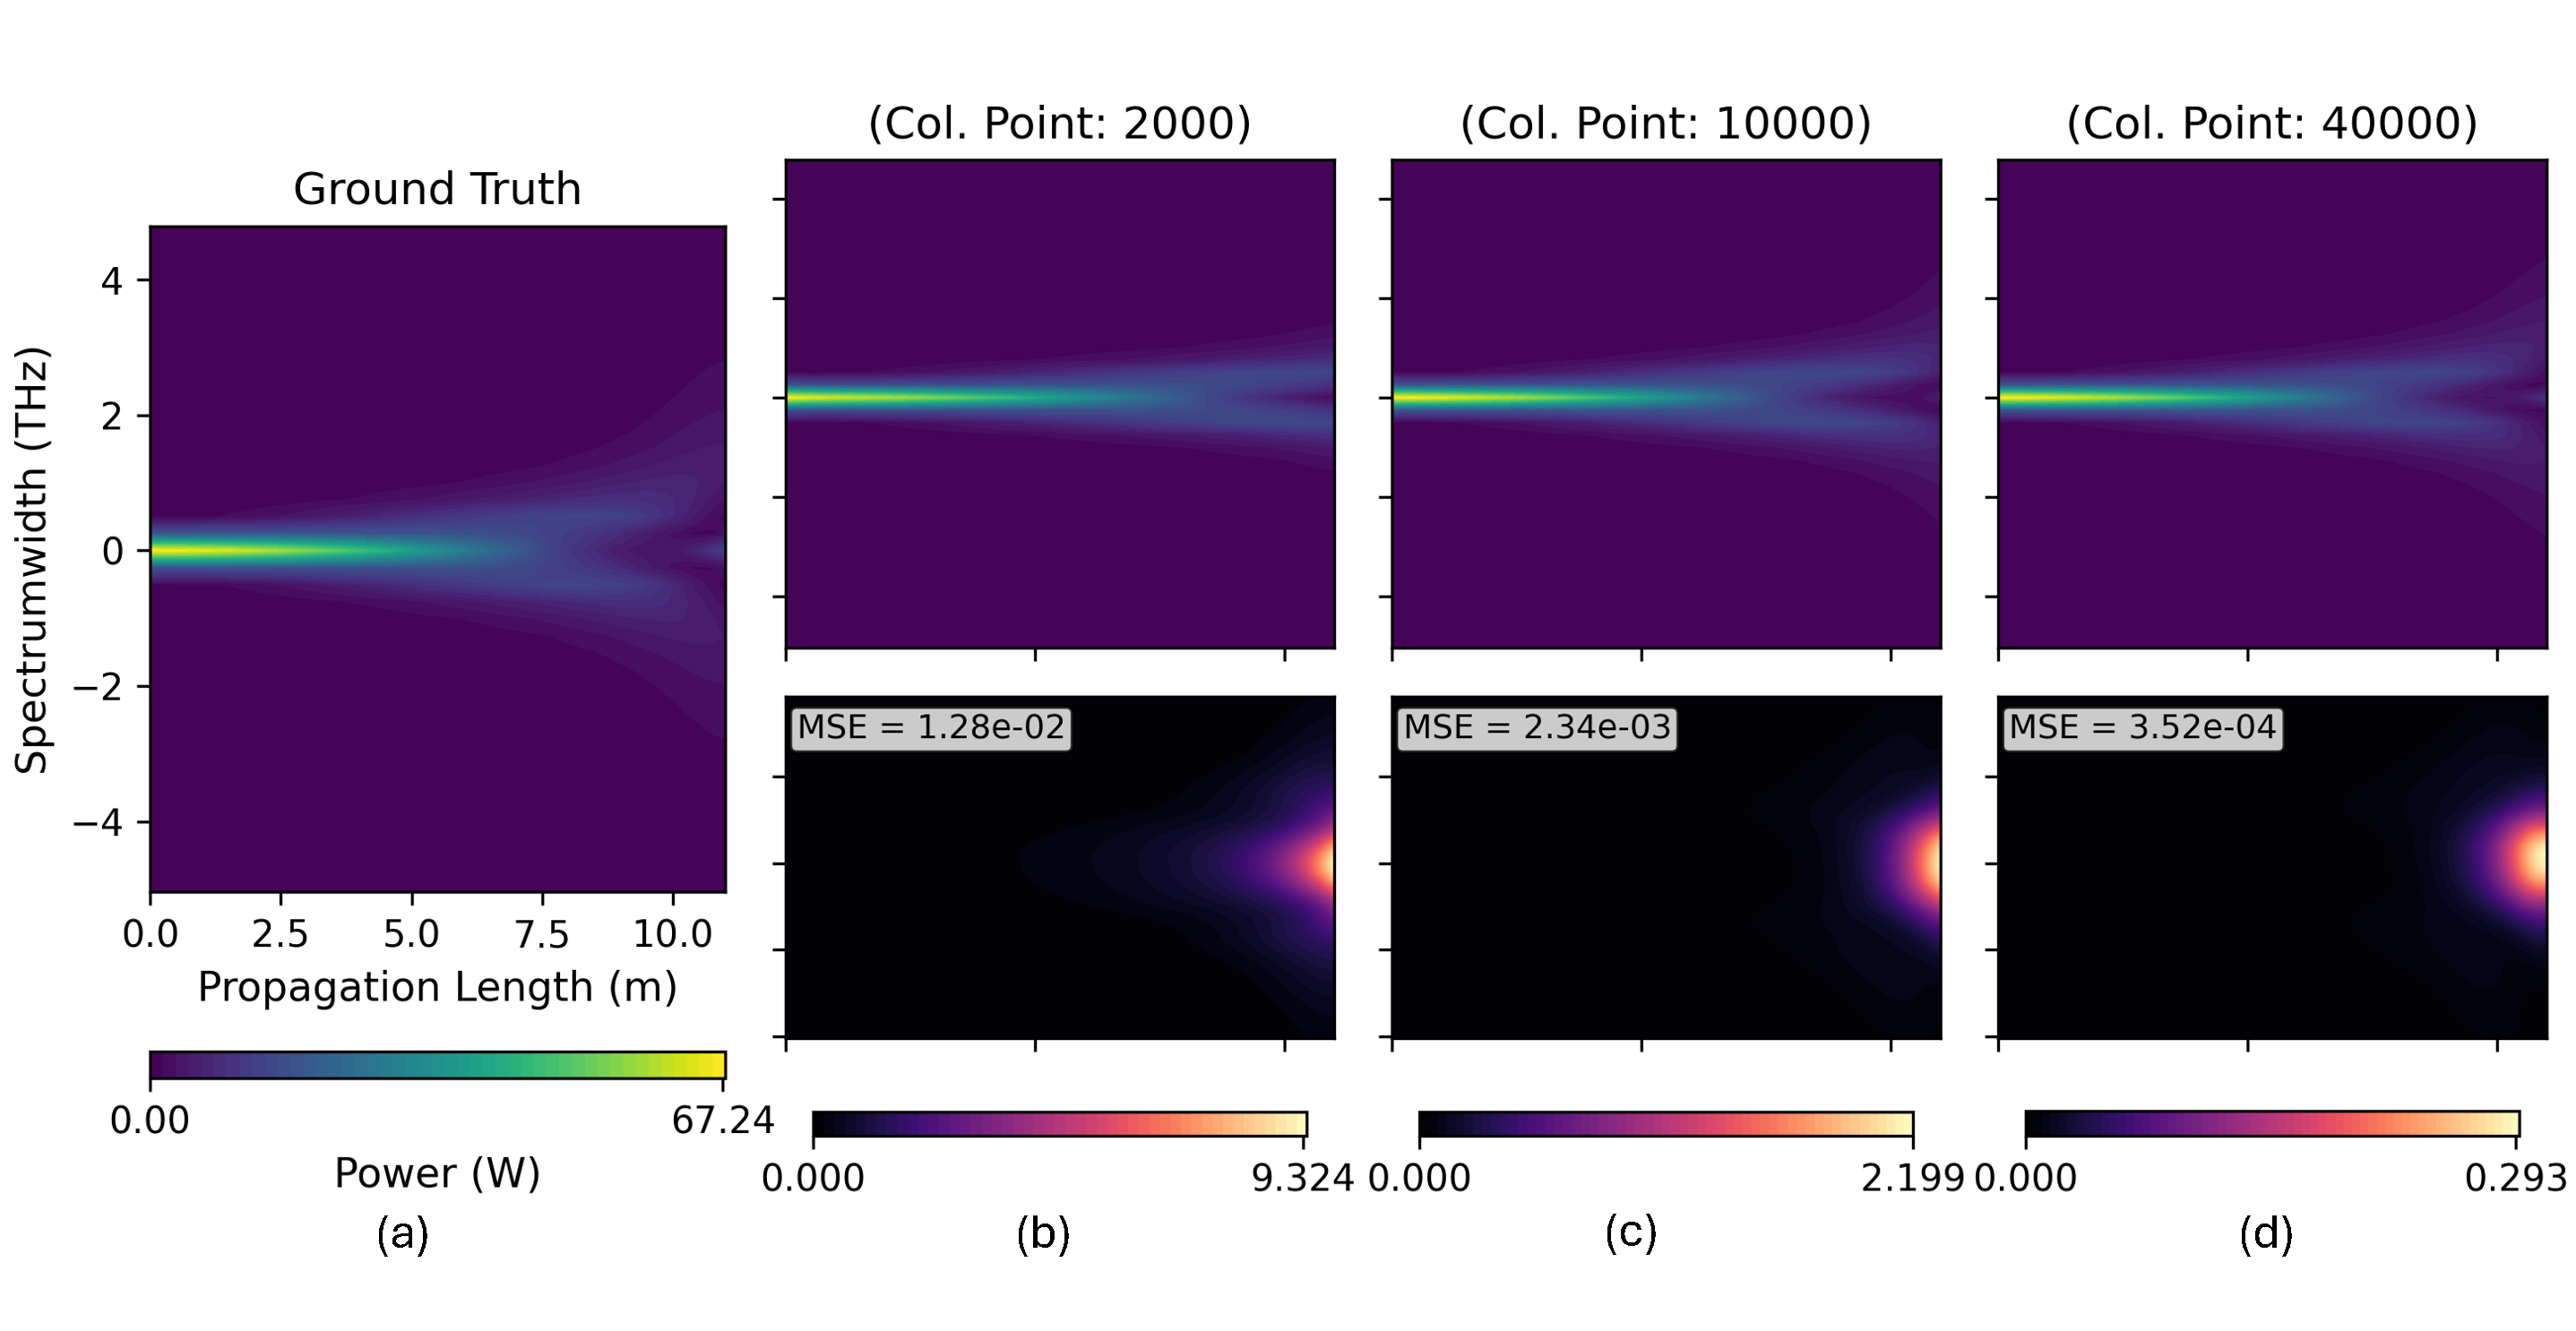
\includegraphics[width=0.9 \linewidth]{Gambar/resultsVanillaS.png}
    \caption{Distribusi daya spektrum (PINNs)}
    (a) Referensi numerik, (b)–(d) Prediksi PINNs dengan Titik Kolokasi 2.000, 5.000, dan 10.000 (atas: daya spektrum; bawah: error prediksi (MSE))
    \label{fig:specPINNs}
\end{figure}

Informasi dari seluruh nilai MSE dari percobaan Vanilla-PINNs terdapat pada Gambar \ref{fig:VPINN-MSE}. Nilai MSE memberikan distribusi yang lebar pada jumlah titik kolokasi 2.000 dan 5.000. Inferensi PINNs dapat menghasilkan prediksi yang baik atau buruk berdasarkan titik kolokasi tersebar. Pada persebaran titik kolokasi yang renggang, model sangat sensitif terhadap bagaimana sampel domain dipilih. Hal ini menyebabkan hasil yang tidak konsisten ketika ketika diujicobakan pada pembelajaran dengan \emph{random seed} yang berbeda.

\newpage

\begin{figure}[htbp]
    \centering
    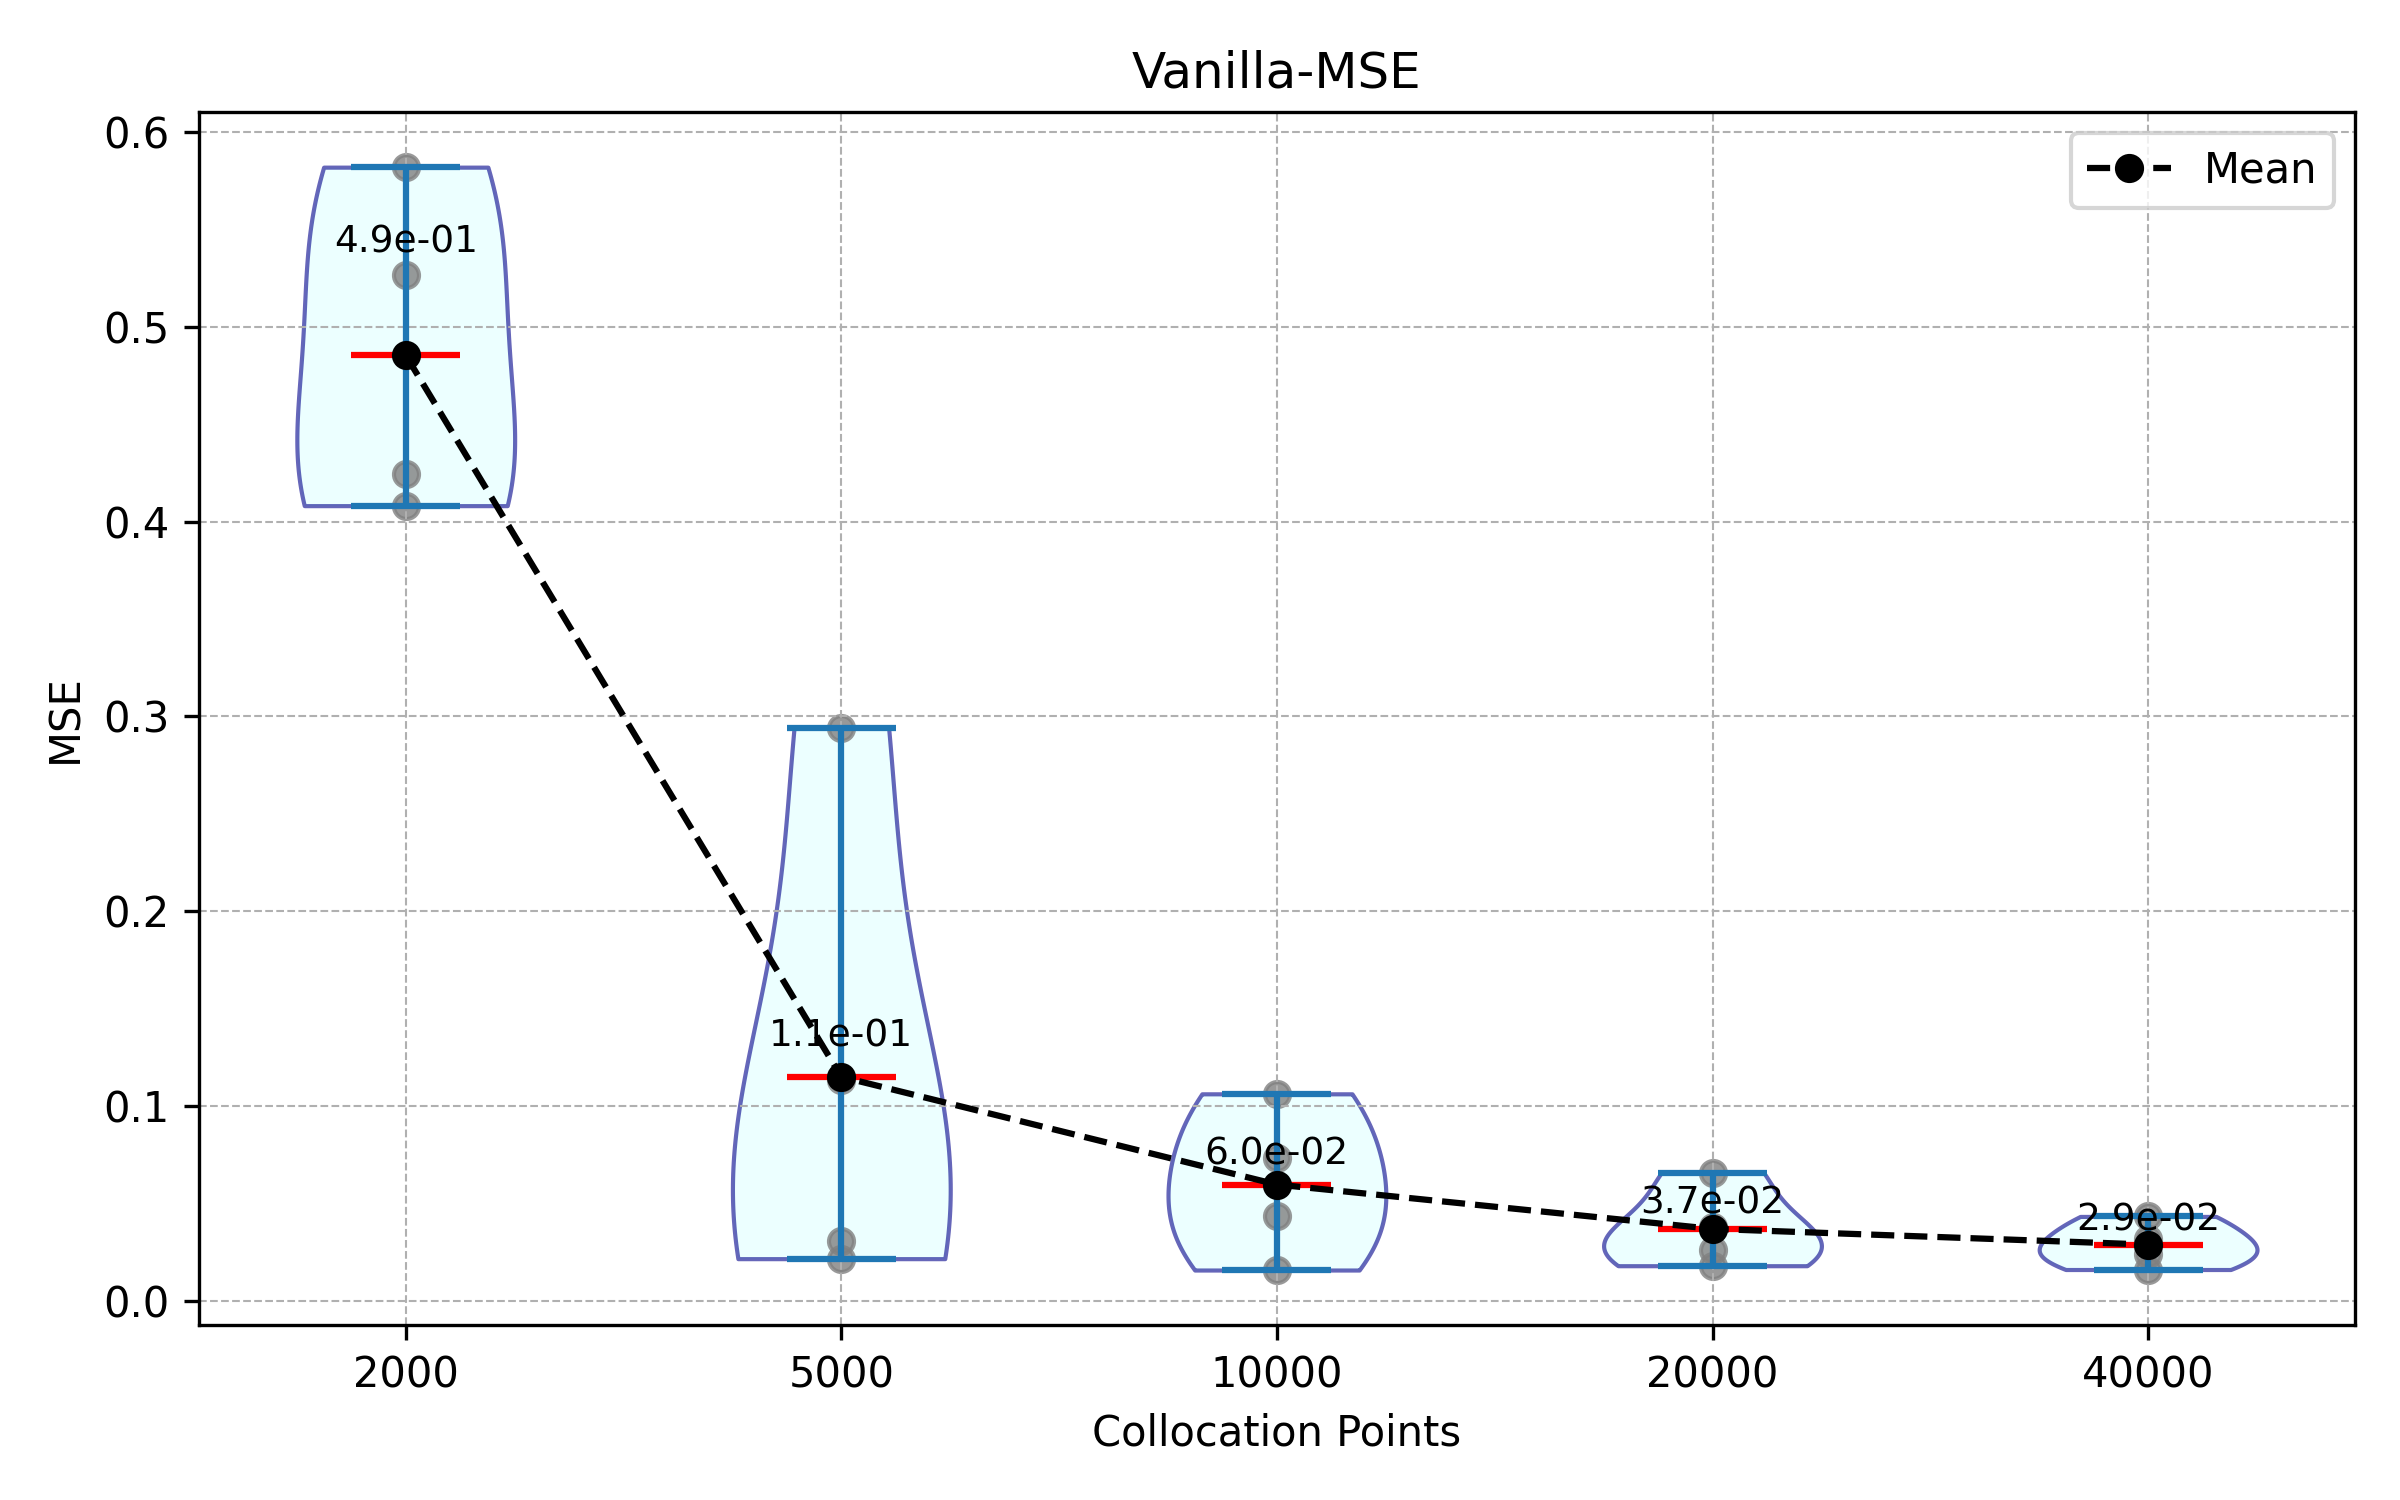
\includegraphics[width=0.9 \linewidth]{Gambar/colPoints-Error.png}
    \caption{Nilai MSE Prediksi Temporal PINNs}
    \label{fig:VPINN-MSE}
\end{figure} 

Sebaliknya, jumlah titik kolokasi yang lebih besar memberikan hasil yang lebih konsisten dengan persebaran nilai MSE yang lebih sempit. Distribusi titik yang menjadi lebih rapat menyebabkan model mendapatkan informasi yang cukup selama pembelajaran. Oleh sebab itu, model dengan 40.000 sampel memiliki tingkat presisi terbaik dari jumlah sampel yang lain. 

Akurasi model dapat diamati melalui rata-rata nilai MSE dalam keempat perulangan. Sebuah garis pada gambar \ref{fig:VPINN-MSE} ditarik terhadap nilai rata-rata MSE pada setiap jumlah kolokasi. Garis tersebut menunjukkan penurunan rata-rata MSE secara eksponensial seiring dengan meningkatnya jumlah sampel. Dapat disimpulkan bahwa konvergensi nilai MSE menunjukkan peningkatan akurasi dan presisi seiring dengan bertambahnya jumlah kolokasi.

Akan tetapi, meningkatkan jumlah sampel kolokasi berpotensi meningkatkan waktu pembelajaran dan kompleksitas komputasi secara signifikan. Hal ini disebabkan oleh bertambahnya jumlah perhitungan residual yang perlu dilakukan model PINNs pada setiap iterasi. Oleh karena itu, pemilihan jumlah titik kolokasi yang optimal menjadi krusial untuk mencapai keseimbangan antara akurasi prediksi dan efisiensi pelatihan.

Proses pembelajaran PINNs dilakukan menggunakan strategi optimasi ADAM dilanjutkan dengan strategi L-BFGS. Optimasi ADAM mengakumulasi gradien dan variansi gradien dari proses optimasi sebelumnya sebagai fungsi momentum. Strategi optimasi ini mampu menyesuaikan proses pembelajaran secara dinamis dan memberikan optimasi yang lebih terarah. Akan tetapi, fungsi biaya residual $\mathcal{H}$ yang melibatkan turunan hingga derajat ketiga menyebabkan gradien numerik dari proses optimasi yang tidak stabil. Hal ini menyebabkan terjadinya fluktuasi yang signifikan pada optimasi ADAM selama 40.000 epoch.

\begin{figure}[htbp]
    \centering
    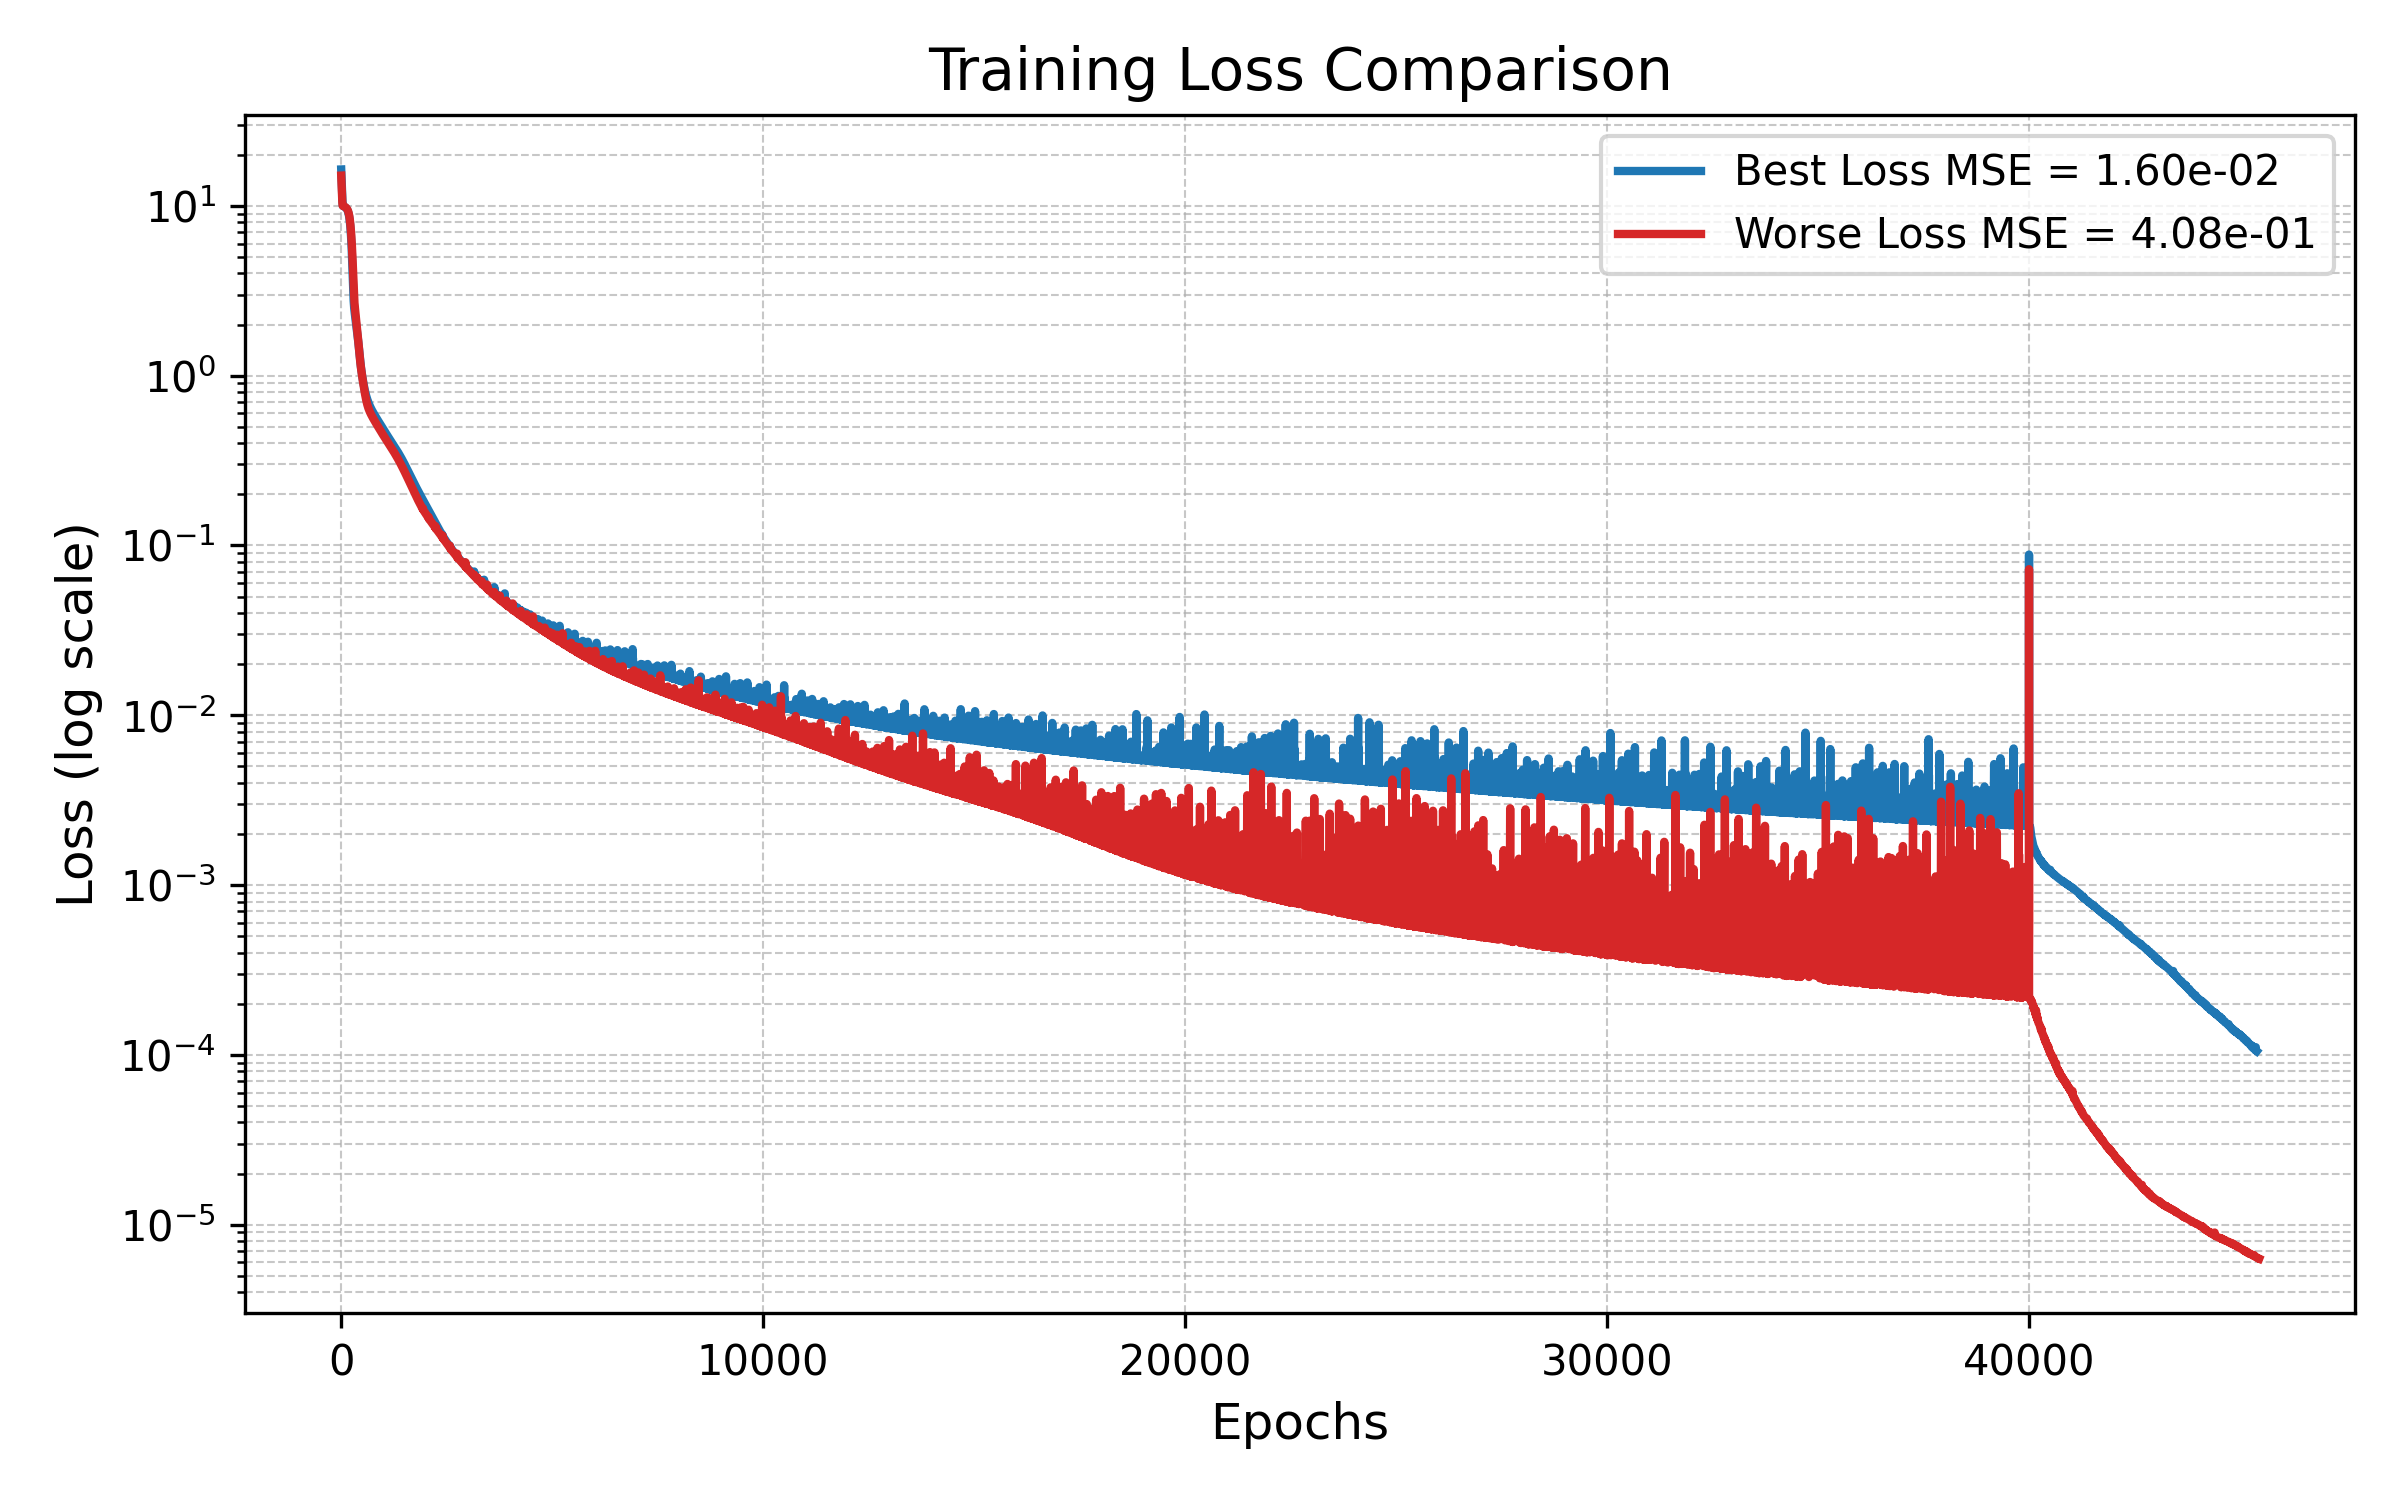
\includegraphics[width=0.9 \linewidth]{Gambar/Loss-Comparison.png}
    \caption{Grafik Fungsi Loss Vanilla-PINNs}
    \label{fig:loss-PINNs}
\end{figure}

Setelah fase awal ADAM, pelatihan dilanjutkan menggunakan algoritma L-BFGS yang bersifat deterministik dan memanfaatkan informasi kurva loss secara global. L-BFGS berperan sebagai metode penyelaman yang secara tajam dan efisien mengarahkan model menuju solusi optimal. Proses penyelaman terlihat dari penurunan \emph{residual loss} yang sangat cepat pada 5.000 epoch terakhir. Namun, L-BFGS memerlukan penggunaan dan penyimpanan matriks Hessian aproksimasi dalam jumlah besar sehingga jumlah epoch perlu dibatasi untuk menjaga efisiensi waktu pelatihan.

Nilai loss pada Gambar \ref{fig:loss-PINNs} menunjukkan bahwa model dengan 2.000 titik collocation memiliki performa konvergensi \emph{residual loss} yang tampak lebih kecil dibandingkan model dengan 40.000 titik. Namun, nilai MSE antara kedua model justru menunjukkan hasil yang bertolak belakang. Seperti yang telah disimpulkan, model dengan jumlah titik kolokasi yang lebih banyak selama pembelajaran memberikan prediksi yang lebih akurat. 

Kontradiksi tersebut dapat dijelaskan dengan fenomena \emph{underfitting} pada model dengan jumlah titik kolokasi yang terlalu sedikit. Dikarenakan cakupan ruang solusi yang terbatas, model dapat dengan mudah menyesuaikan diri pada titik tersebut tanpa benar-benar memahami perilaku fisis dari solusi sebenarnya. Akibatnya, meskipun \emph{residual loss}—yang dihitung hanya pada titik-titik tersebut terlihat kecil, model gagal melakukan generalisasi dengan baik, yang tercermin pada nilai MSE yang tinggi ketika diuji terhadap solusi sebenarnya.

\section {Evaluasi Hasil Prediksi SAS-PINNs}
SMOTE merupakan salah satu teknik \emph{oversampling} yang digunakan untuk menyeimbangkan distribusi data minoritas dengan data mayoritas dalam proses klasifikasi. Akan tetapi, pada strategi SAS-PINNs, SMOTE digunakan untuk memfokuskan titik kolokasi tambahan pada area dengan kesulitan konvergensi tinggi. Kedua parameter SAS-PINNs memiliki peranan masing-masing. Nilai Ambang menyatakan luas area penambahan data di mana semakin kecil nilainya, \emph{oversampling} akan dilakukan pada area dengan residual tertinggi secara lebih terfokus. Rasio \emph{Oversampling} menyatakan seberapa banyak data yang akan ditambahkan melalui perbandingan dari target data minoritas terhadap data mayoritas.

Secara konvensional, SMOTE digunakan untuk menyeimbangkan jumlah data minoritas terhadap data mayoritas. Hal ini dilakukan dengan mengatur rasio \emph{oversampling} sebagai satu yang menghasilkan perbandingan jumlah data minoritas dan mayoritas menjadi 1:1. Akan tetapi, SAS-PINNs memiliki paradigma yang berbeda di mana SMOTE tidak digunakan untuk menyeimbangkan titik kolokasi. Gambar \ref{fig:Bad-SAS-PINNs} menunjukkan apa yang terjadi pada inferensi model jika jumlah rasio \emph{oversampling} diatur sebagai 1 untuk tiap nilai ambang pada titik kolokasi 10.000.


\begin{figure}[htbp]
    \centering
    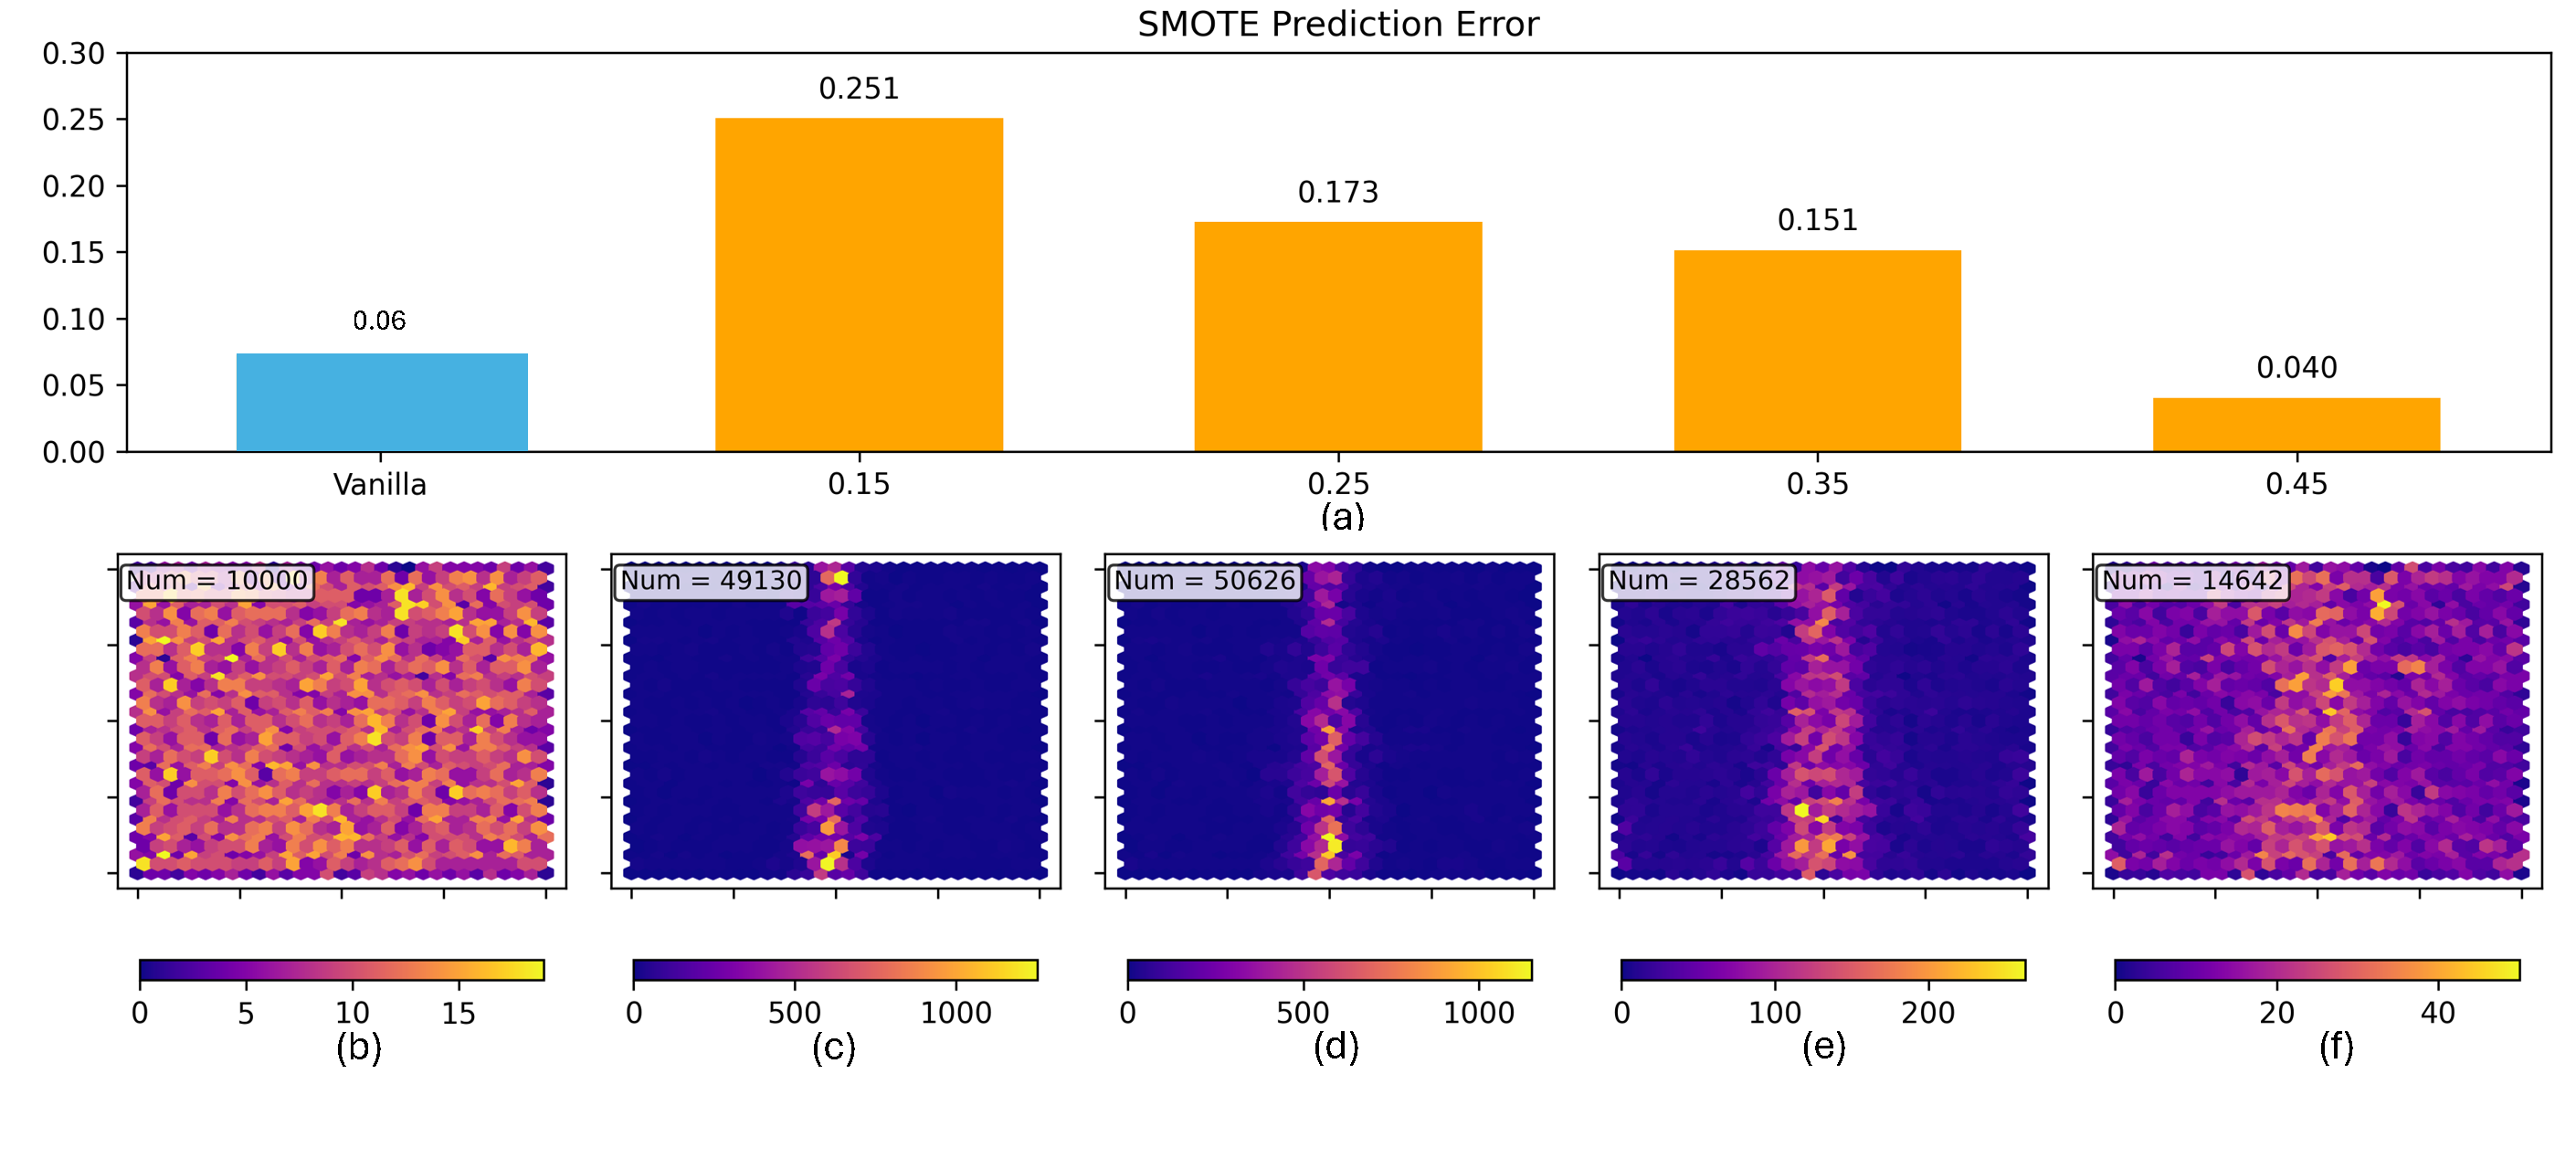
\includegraphics[width=0.9 \linewidth]{Gambar/smoteDistribution.png}
    \caption{Nilai MSE SAS-PINNs dengan Rasio 1}
    (a) Rata-Rata MSE Vanilla-PINNs dan MSE SAS-PINNs untuk Empat Perlakuan Nilai Ambang; (b) Distribusi Sampel Vanilla-PINNs; (c)-(f) Distribusi Sampel SAS-PINNs pada Nilai Ambang 0.15, 0.25, 0.35, 0.45
    \label{fig:Bad-SAS-PINNs}
\end{figure}

Dengan mengatur nilai rasio sebagai 1, jumlah titik kolokasi yang ditambahkan menjadi tidak terkontrol pada nilai ambang yang kecil. Sebagai contoh, pada nilai ambang 0.15, sebanyak 39.130 titik ditambahkan pada area dengan residual tertinggi. Hal ini justru merusak distribusi data secara signifikan, di mana mula-mula model hanya memiliki 10.000 titik kolokasi yang tersebar seragam. Rusaknya distribusi data mengakibatkan model tidak dapat melakukan konvergensi pada keseluruhan domain secara menyeluruh, menyebabkan peningkatan nilai MSE yang mencapai 0.251.

Akan tetapi, permasalahan ini tidak ditunjukkan pada nilai ambang 0.45, di mana hanya 4.642 data yang ditambahkan ke dalam model. Penambahan data ini terbukti menurunkan nilai MSE menjadi 0.04. Oleh karena itu, pengaturan rasio \emph{oversampling} perlu mempertimbangkan nilai ambang yang digunakan, di mana semakin kecil nilai ambang, perlu digunakan angka rasio yang lebih kecil. Informasi ini menjadi alasan atas digunakannya konfigurasi nilai ambang dan rasio sebagai berikut:

\begin{table}[htbp]
    \centering
    \begin{threeparttable}
        \caption{Nilai Ambang dan Rasio SAS-PINNs}
        \begin{tabular}{|p{5cm}|p{4cm}|}
				\hline
				Nilai Ambang & Rasio \\
                \hline 
                0.45 & 1\\
                \hline
                0.35 & 0.7 \\
                \hline
                0.25 & 0.4 \\
                \hline
                0.15 & 0.25 \\
                \hline
			\end{tabular}
        \label{SAS-config}
    \end{threeparttable}
\end{table} 

\begin{figure}[htbp]
    \centering
    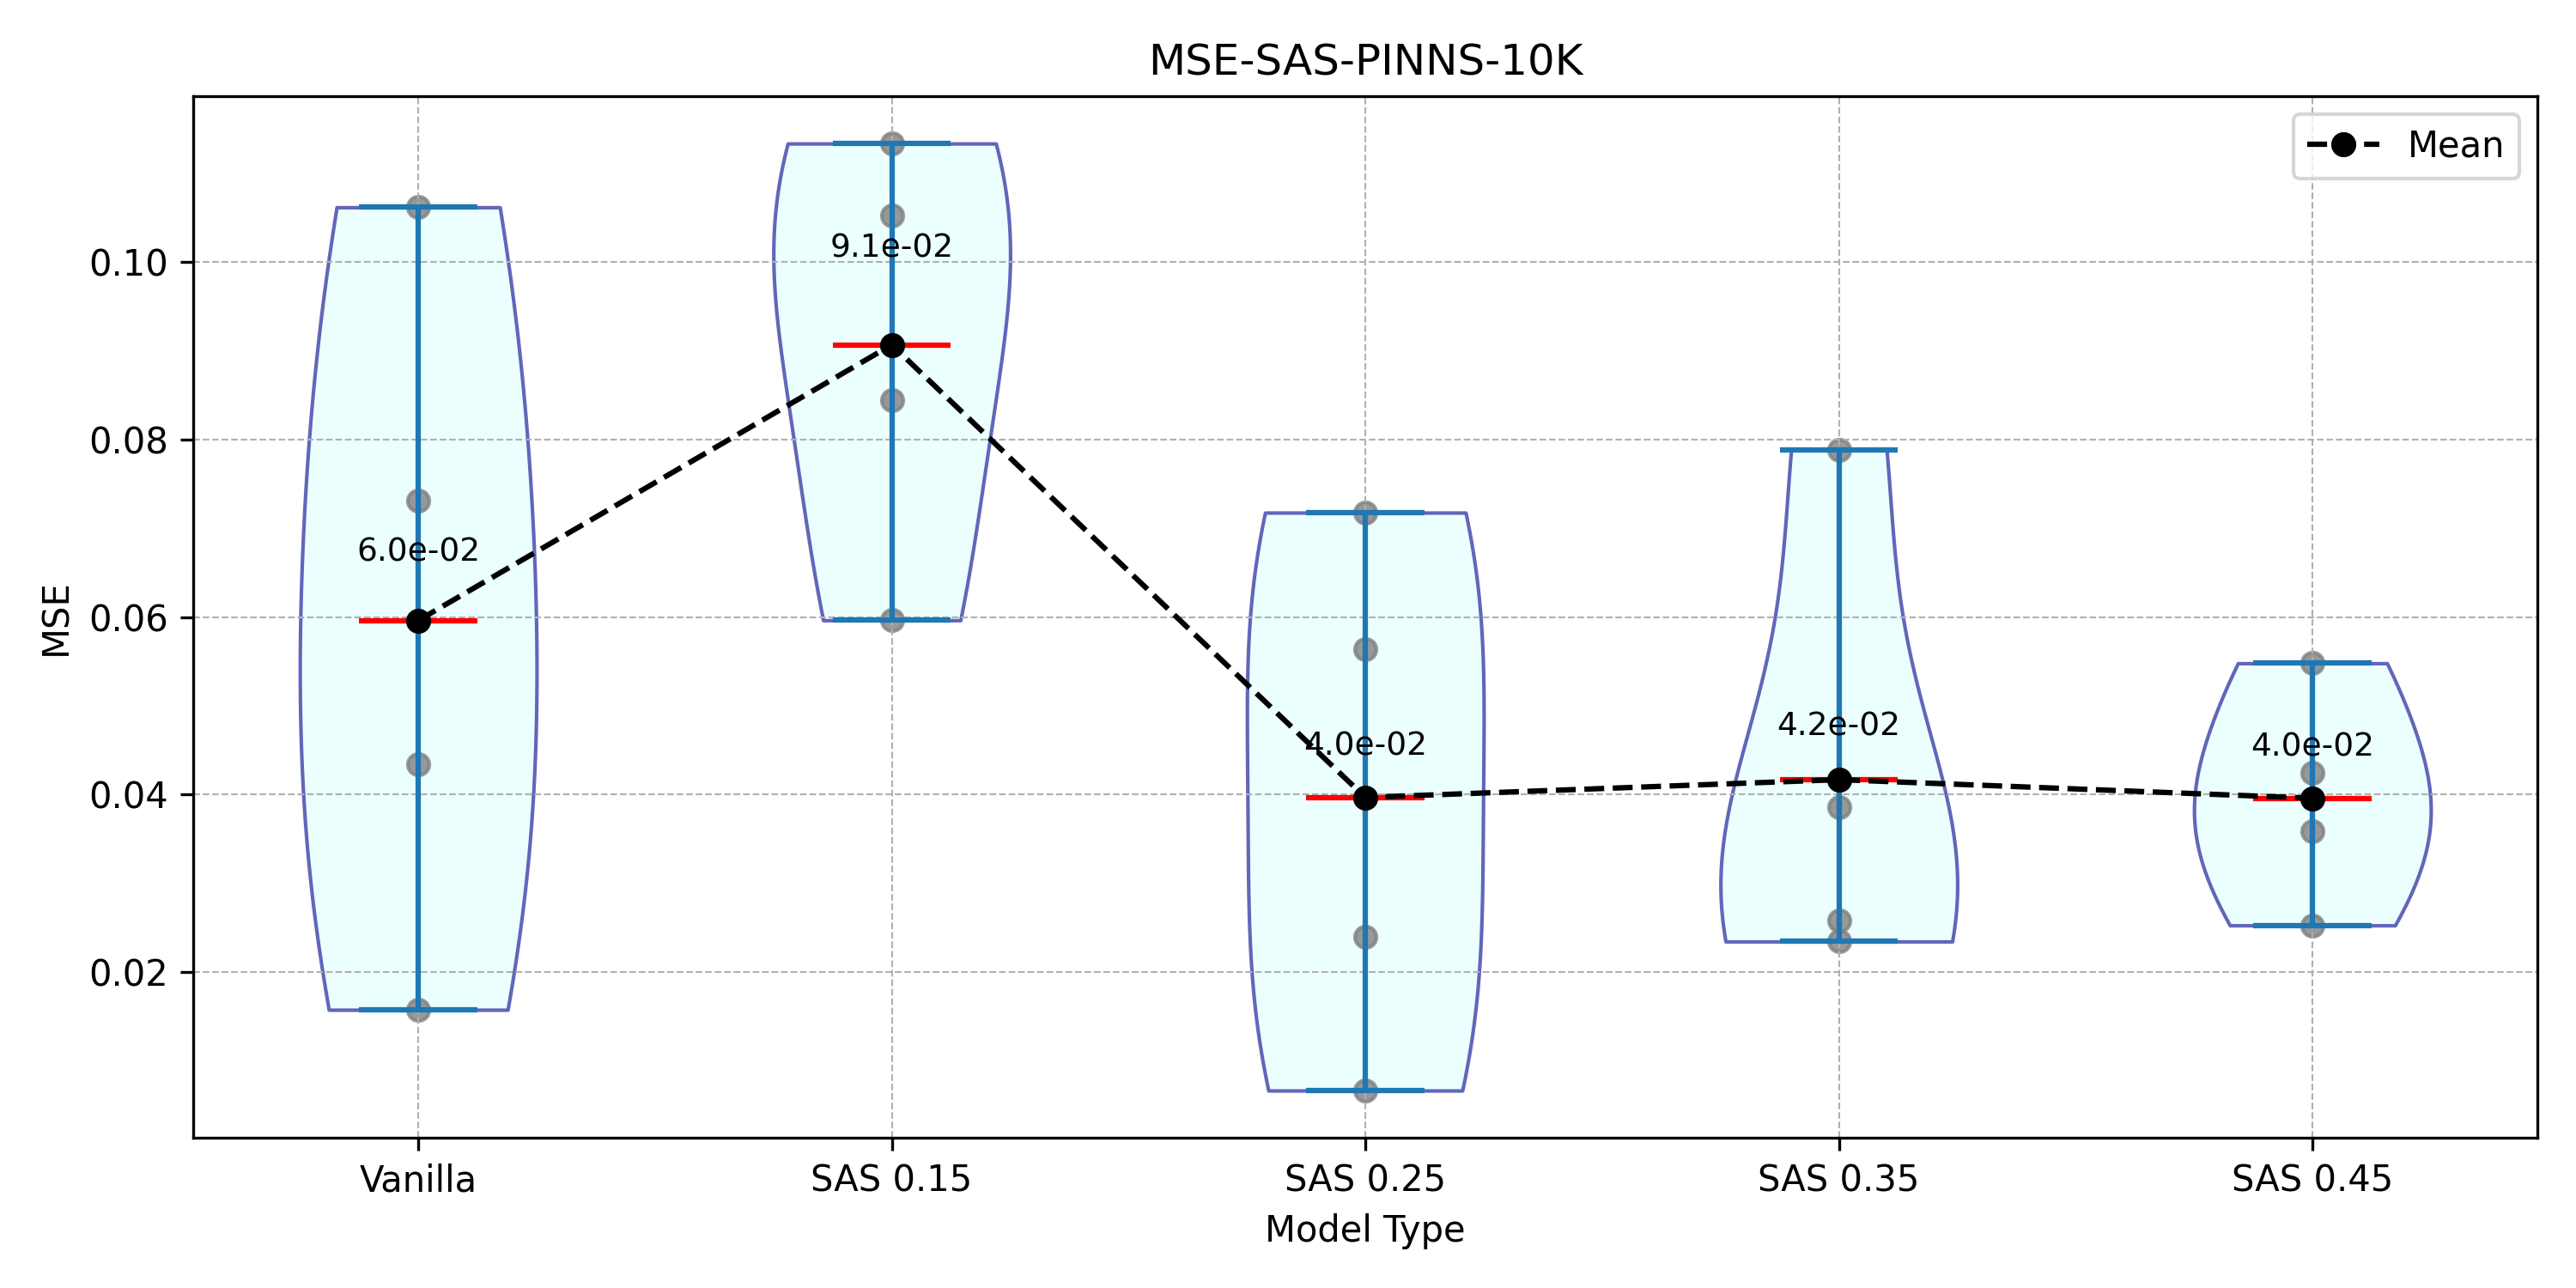
\includegraphics[width=1 \linewidth]{Gambar/smoteDistribution-All.png}
    \caption{Perbandingan MSE Vanilla-PINNs vs SAS-PINNs}
    \label{fig:Good-SAS-PINNs}
\end{figure}

Evaluasi MSE SAS-PINNs diberikan pada Gambar \ref{fig:Good-SAS-PINNs}. Model SAS-PINNs dibandingkan dengan model Vanilla-PINNs yang dilatih pada sampel kolokasi yang sama sejumlah 10.000 titik. Rata-rata MSE dari model Vanilla berada pada angka 0.06. Model SAS-PINNs pada nilai ambang 0.25--0.45 berdasarkan konfigurasi \ref{SAS-config} menunjukkan penurunan pada angka MSE rata-rata, masing-masing yakni, 0.04, 0.042, dan 0.04. Akan tetapi, pada nilai ambang 0.15, nilai MSE rata-rata justru meningkat menjadi 0.091.


\begin{figure}[htbp]
    \centering
    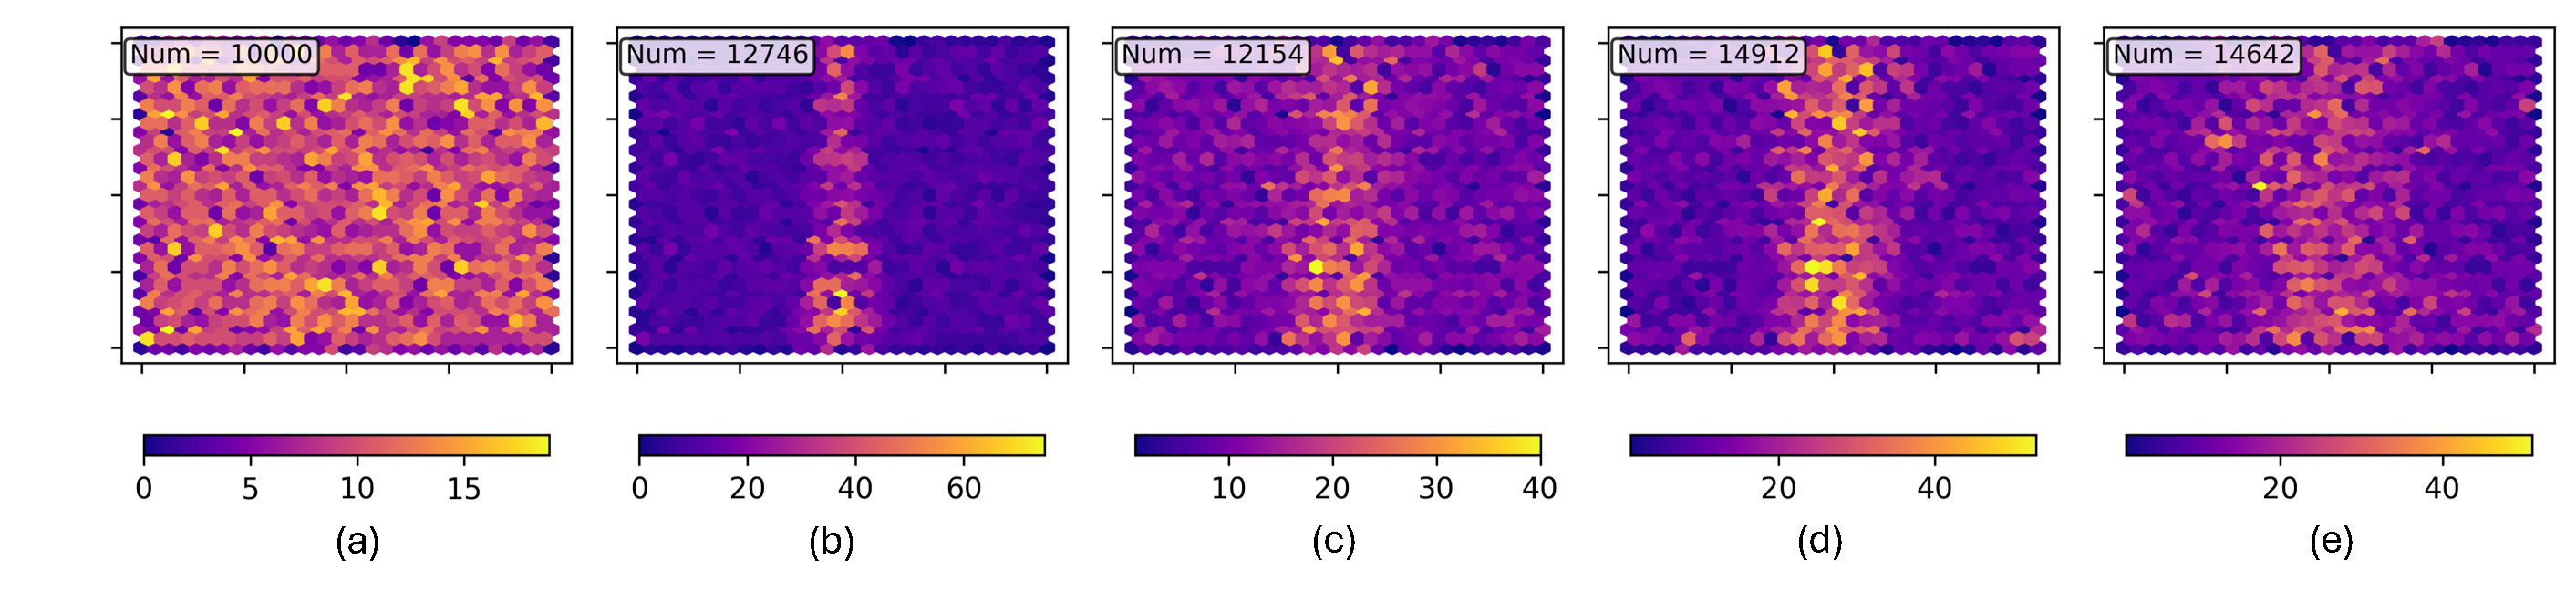
\includegraphics[width=1 \linewidth]{Gambar/colSMOTE.png}
    \caption{Distribusi Sampel SAS-PINNs Terkonfigurasi}
    (a) Titik Kolokasi Vanilla-PINNs; (b)-(e) Titik Kolokasi SAS-PINNs pada Keempat Tipe Konfigurasi Tabel \ref{SAS-config}
    \label{fig:col-SAS-PINNs}
\end{figure}

Konfigurasi nilai ambang 0.15 memberikan augmentasi titik yang terfokus. Walaupun hanya sejumlah 2.746 titik yang ditambahkan, kawasan penambahan titik yang terlalu terpusat pada 15\% zona residual tertinggi terbukti berdampak buruk terhadap konvergensi PINNs. Di lain sisi, penambahan titik dengan jumlah yang serupa (2.154 titik) pada 25\% zona residual tertinggi justru mampu memperbaiki konvergensi model. Sementara itu, pengaturan nilai ambang 0.45 memberikan persebaran titik tambahan yang lebih luas, tetapi menghasilkan presisi terbaik dari model SAS-PINNs yang lain. 

Dapat disimpulkan bahwa strategi penambahan titik yang paling optimal didapatkan ketika nilai ambang SAS-PINNs cukup besar. Hal ini menyebabkan penambahan titik dilakukan pada area yang lebih luas. Penambahan selektif ini memungkinkan model memfokuskan kapasitasnya pada daerah tertentu, dengan tetap menjaga cakupan global domain fisis. Akan tetapi, nilai ambang yang terlalu kecil berpotensi membuat model terlalu selektif sehingga kehilangan informasi penting dari domain lainnya. 

Hal ini dibuktikan pada Gambar \ref{fig:loss-SAS-PINNs}, di mana penambahan titik kolokasi menyebabkan nilai loss meningkat secara periodik setiap 10.000 epoch. Akan tetapi, pada strategi nilai ambang sampling 0.15, peningkatan periodik ini menjadi sangat signifikan sehingga konvergensi proses pembelajaran menjadi stagnan. Akibatnya, pada proses optimasi L-BFGS, model tidak dapat melakukan konvergensi sebaik model SAS-PINNs dengan nilai ambang 0.45, maupun dengan model Vanilla-PINNs.

\begin{figure}[htbp]
    \centering
    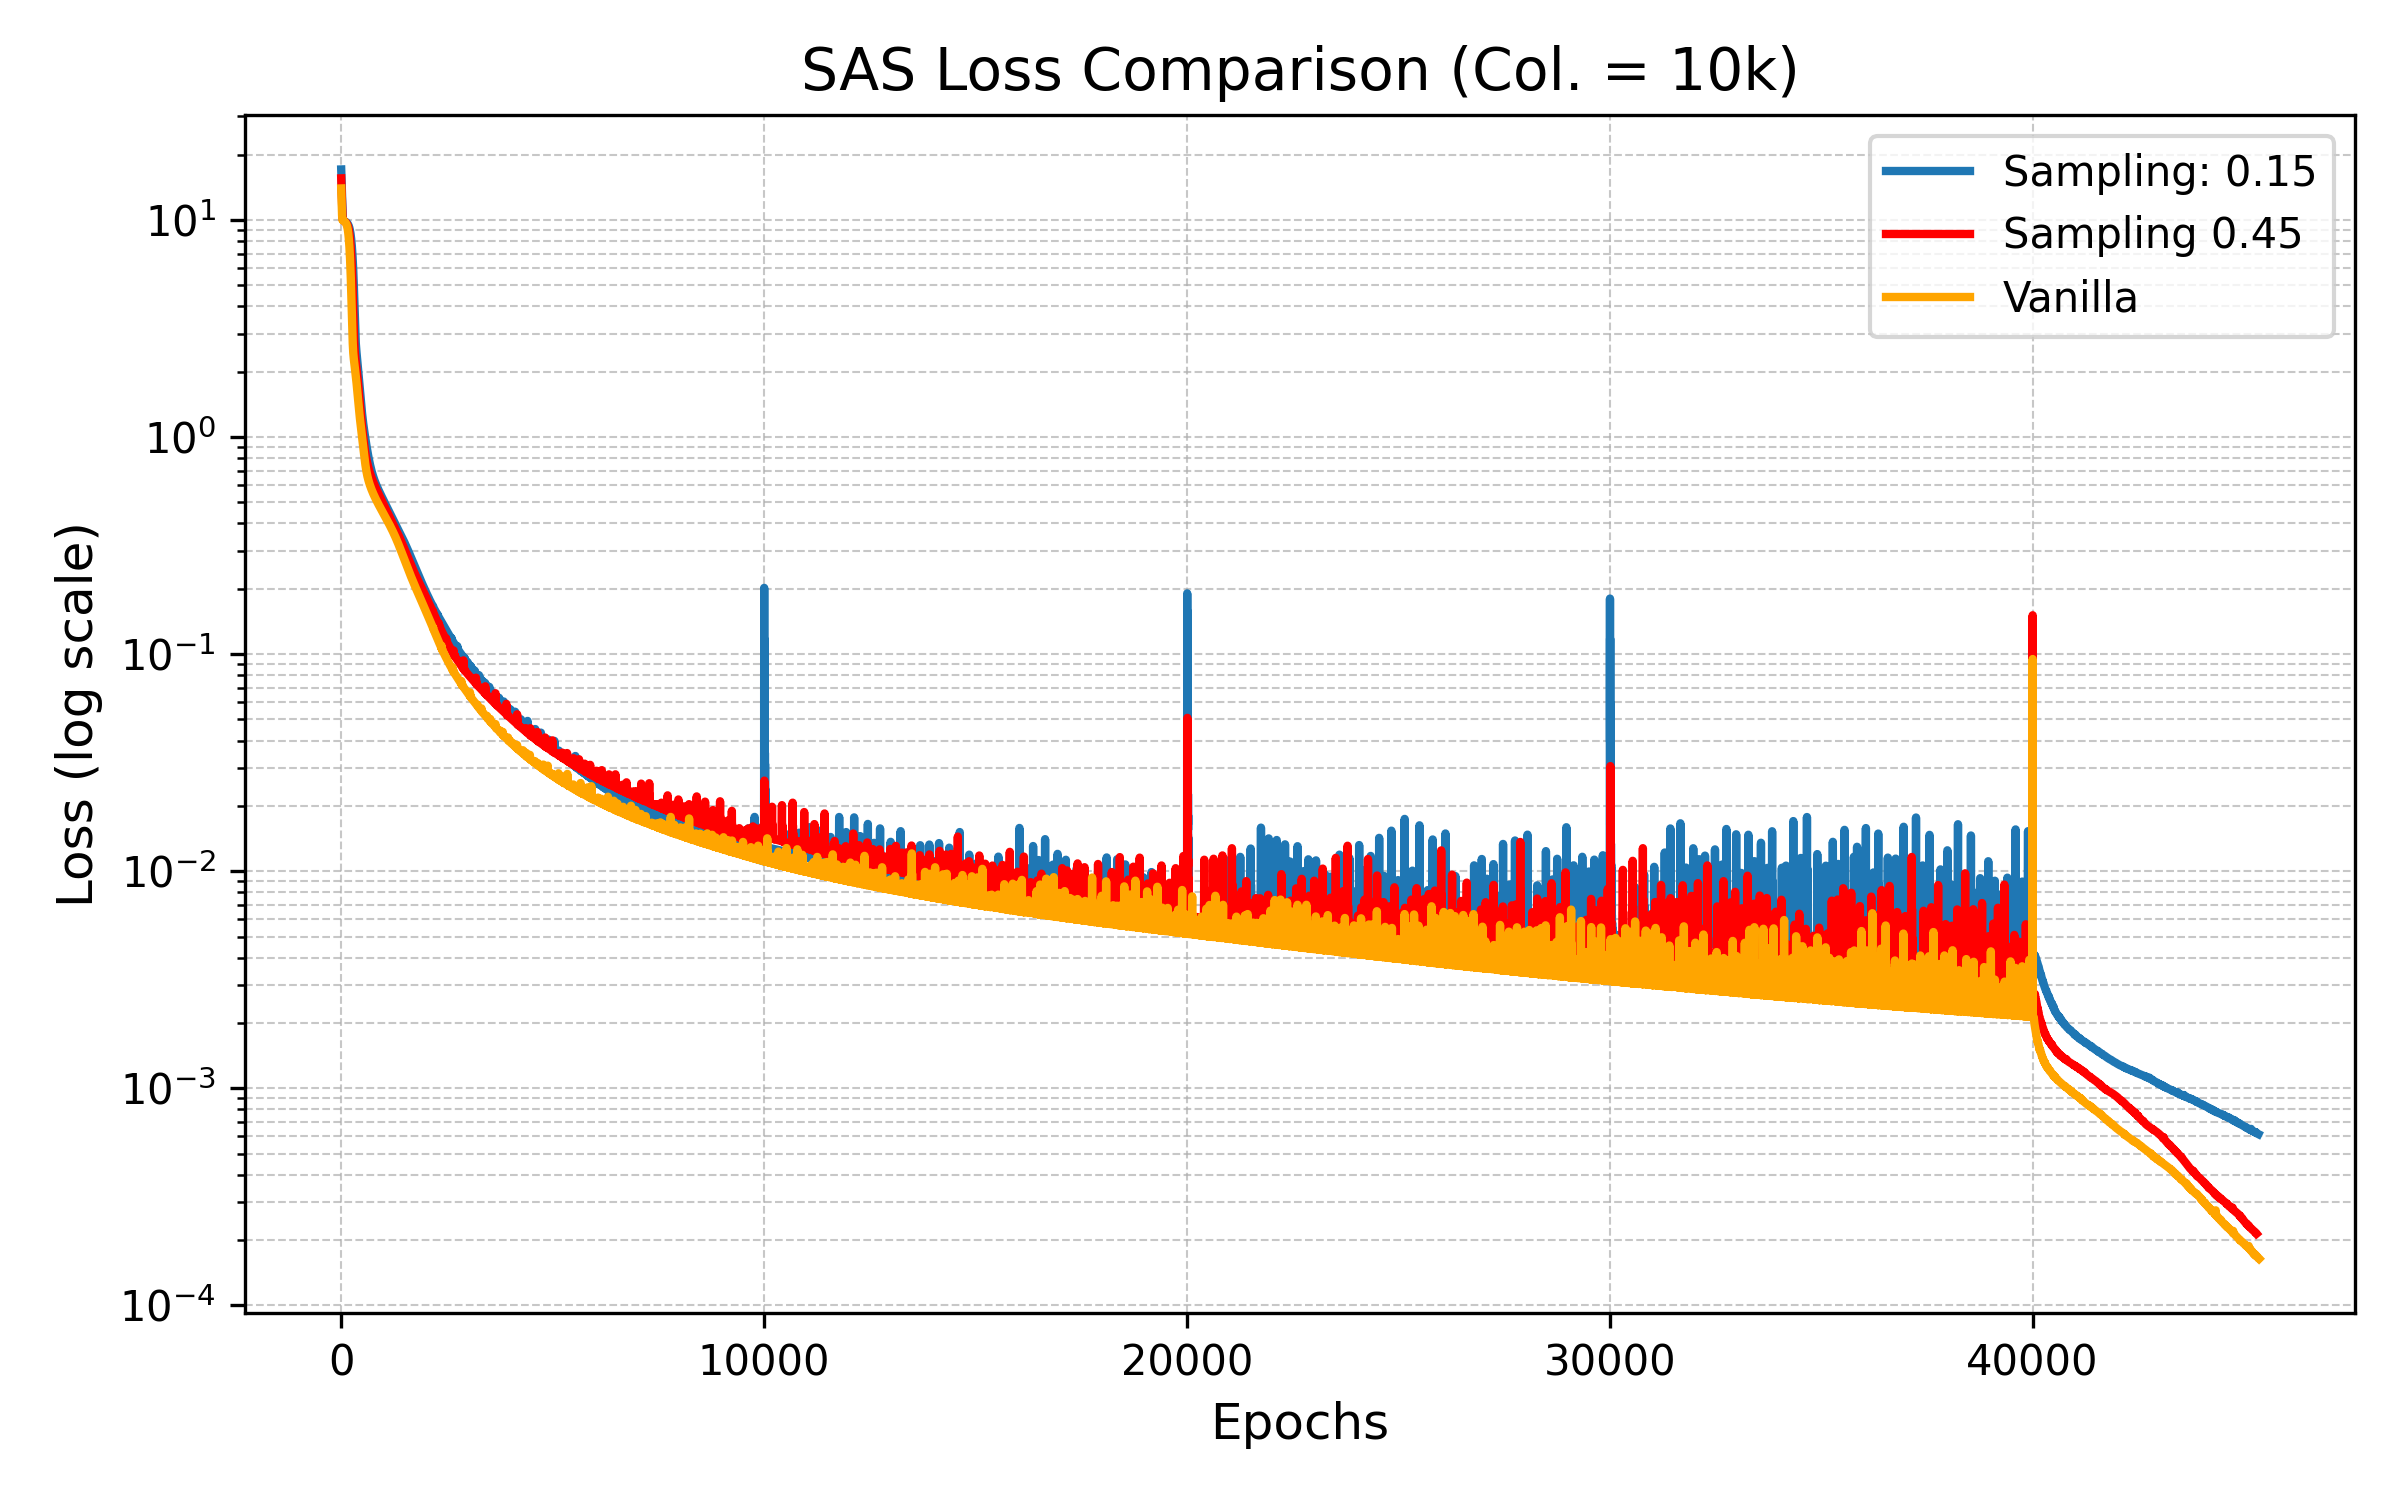
\includegraphics[width=0.8 \linewidth]{Gambar/SASLoss-Comparison (1).png}
    \caption{Perbandingan Konvergensi Loss Model}
    \label{fig:loss-SAS-PINNs}
\end{figure}

%%%%%%%%%%%%%%%%%%%%%%%%%%%%%%%%%%%%%%%%%%%%%%%%%%%%%%%%%%%%%%
\cleardoublepage
	\addtocontents{toc}{\protect\addvspace{5pt}}
\chapter{PENUTUP}

\section{Kesimpulan}

Berdasarkan hasil penelitian yang dilakukan, dapat disimpulkan bahwa: 

\begin{enumerate}

    \item \emph{Physics-Informed Neural Networks} (PINNs) mampu menyelesaikan persamaan Schr\"{o}dinger Nonlinear (NLS) dalam kasus pulsa \emph{ultrashort}. Metode ini memerlukan normalisasi persamaan untuk menjaga stabilitas numerik. Model menggunakan empat lapisan tersembunyi dengan masing-masing 128 neuron, fungsi aktivasi $\tanh()$, dan strategi optimasi ADAM-LBFGS. Model dites pada variasi jumlah titik kolokasi dan variasi angka \emph{random seed}

    \item Evaluasi Pendekatan Vanilla-PINNs terhadap referensi data \emph{Split-Step Fourier Method} (SSFM) menunjukkan kemampuan prediksi model yang meningkat secara eksponensial dengan jumlah titik kolokasi yang digunakan. 

    \item SAS-PINNs (SMOTE Adaptive Sampling) berhasil meningkatkan akurasi dan konsistensi prediksi dengan mengonfigurasi Nilai Ambang dan Rasio \emph{Oversampling}. Namun, konsentrasi penambahan titik yang terlalu terfokus (niai ambang kecil) berpotensi mengganggu generalisasi model.
    
\end{enumerate}

\newpage
\section{Saran}
Disarankan untuk mengeksplorasi teknik \emph{SMOTE-Adaptive Sampling} (SAS) dengan beberapa modifikasi pelatihan adaptif seperti pendekatan dekomposisi domain maupun penerapan \emph{causal training}.  Kombinasi ini diharapkan meningkatkan performa PINNs dengan mempertimbangkan urutan temporal data.
	
	\backmatter
	% Daftar Pustaka tanpa halaman kosong berlebih
\cleardoublepage                                % Mulai di halaman baru, aman untuk 2-sisi
\phantomsection                                 % 

%Format Daftar Pustaka (Biblio)
% Format dan ganti judul daftar pustaka
\makeatletter 
\renewcommand\@biblabel[1]{} % Hilangkan numbering
\makeatother
\parindent 0cm
\parskip 0.1cm
\renewcommand{\bibname}{DAFTAR PUSTAKA}  % Ganti judul default dari "Bibliografi" atau "References"

\bibliographystyle{apacite}                    % Gaya sitasi
\bibliography{references}                      % File .bib

	\chapter*{LAMPIRAN}
\addcontentsline{toc}{chapter}{LAMPIRAN}
\renewcommand{\thetable}{L\theappendix\arabic{table}}
\renewcommand{\thefigure}{L\theappendix\arabic{figure}}
\renewcommand{\theequation}{L\theappendix\arabic{equation}}
\myappendix{Penurunan Persamaan Non-Linear Schrodinger}

Penurunan persamaan ini diberikan dalam \citeA{agrawal2019nonlinear}.

Empat Persamaan Maxwell diberikan untuk menggambarkan fenomenda dari perambatan pulsa optik serat sebagai berikut: 

\begin{equation}
    \nabla \times \vec{E} = - \frac{\partial \vec{B}}{\partial t}
\end{equation}

\begin{equation}
    \nabla \times \vec{B} = \vec{J}+\frac{\partial \vec{D}}{\partial t}
\end{equation}

\begin{equation}
    \nabla \cdot \vec{D} = \rho_f
\end{equation}

\begin{equation}
    \nabla \cdot \vec{B} = 0
\end{equation}

di mana densitas fluks medan listrik \(\vec{D}\) dan medan magnet \(\vec{B}\) dinyatakan dalam: 

\begin{equation}
    \vec{D} = \varepsilon_0\vec{E} + \vec{P}
\end{equation}

\begin{equation}
    \vec{B} = \mu_0 \vec{H} + \vec{M}
\end{equation}

Polarisasi magnet \(\vec{M}\) pada serat optik dinyatakan sebagai 0. Nilai \(\vec{J}\) dan \(\rho_f\) juga dapat dinyatakan sebagai 0 oleh karena muatan bebas dalam serat optik dapat dianggap tidak ada. Mengambil \emph{curl} dari persamaan L.1.1, dan mengubah nilai \(B\) dan \(D\) dari persamaan L.1.5 DAN L.1.6, didapatkan: 

\begin{equation}
    \nabla \times \nabla \times \vec{E} = -\frac{1}{c^2}\frac{\partial \vec{E}^2}{\partial t^2} - \mu_0\frac{\partial \vec{P}^2}{\partial t^2}
\end{equation}

Polarisasi induksi pada serat optik tersusun dari dua bagian yang berupa Polarisasi linear \(\vec{P_L}\) dan polarisasi nonlinear \(\vec{P_{NL}}\)., mengubah persamaan L1.7 sebagai:

\begin{equation}
    \nabla \times \nabla \times \vec{E} = -\frac{1}{c^2}\frac{\partial \vec{E}^2}{\partial t^2} - \mu_0 \left( \frac{\partial \vec{P_L}^2}{\partial t^2} + \frac{\partial \vec{P_{NL}}^2}{\partial t^2} \right)
\end{equation}.

Fungsi medan listrik \(\vec{E}, \vec{P_L}, \vec{P_{NL}}\) dapat dinyatakan terhadap amplitudenya yang berubah dengan perlahan terhadap waktu, relatif terhadap periode optik, sebagai: 

\begin{equation}
    \vec{E}(r,t) = \frac{1}{2}\hat{x}(\mathcal{E}(r,t)\exp(-i\omega_0t)+C)
\end{equation}

\begin{equation}
    \vec{P_L}(r,t) = \frac{1}{2}\hat{x}(\mathcal{P}_L(r,t)\exp(-i\omega_0t)+C)
\end{equation}

\begin{equation}
    \vec{P_{NL}}(r,t) = \frac{1}{2}\hat{x}(\mathcal{P}_{NL}(r,t)\exp(-i\omega_0t)+C)
\end{equation}

dengan komponen polarisasi linear dinyatakan atas: 

\begin{align}
    \mathcal{P}_L(r,t) &= \varepsilon_0 \int_{-\infty}^\infty \chi_{\chi\chi}^1(t-t')\mathcal{E}(r,t')\exp(i\omega_0(t-t') dt' \\
    &= \frac{\varepsilon_0}{2\pi}\int_{-\infty}^\infty \chi_{\chi\chi}^1(\omega)\tilde{\mathcal{E}}(r,\omega-\omega_0)\exp(i(\omega-\omega_0)) dt'
\end{align}

di mana \(\tilde{\mathcal{E}}(r,\omega)\) merupakan transformasi Fourier dari \(\mathcal{E}(r,t)\).

semenatara komponen Polarisasi Nonlinear diberikan dengan 

\begin{equation}
    \mathcal{P}_{NL} \approx \varepsilon_0 \varepsilon_{NL} \mathcal{E}(r,t)
\end{equation}

Untuk mendapatkan nilai dari \(\mathcal{E}(r,t)\), lebih baik untuk bekerja dalam domain Spektral menggunakan transformasi Fourier atas \(\tilde{\mathcal{E}}(r,\omega-\omega_0)\)nyang diberikan sebagai: 

\begin{equation}
    \tilde{\mathcal{E}}(r,\omega) = \int_{-\infty}^{\infty} \mathcal{E}(r,t) \exp(i(\omega-\omega_0)t)dt
\end{equation}

yang mana merupakan solusi dari Persamaan Helmholtz 
\begin{equation}
    \nabla^2\tilde{\mathcal{E}} + \varepsilon(\omega)k_0^2\tilde{\mathcal{E}} =0
\end{equation}

\(k_0\) adalah konstanta dielektrik yang digunakan dalam mendefinisikan refraksi indeks \(\tilde{n}\) dan koefisien absorpsi \(\tilde{\alpha}\).

Separasi variabel dari persamaan L1.15 memberikan: 

\begin{equation}
    \tilde{\mathcal{E}}(r,\omega-\omega_0) = F(x,y)\tilde{A}(z,\omega-\omega_0) \exp(i\beta_0z)
\end{equation}

Kemudian, mengembalikan persamaan L1.16 pada Persamaan Helmholtz memberikan \(F(x,y)\) dan \(\tilde{A}(z,\omega)\)

\begin{equation}
    \frac{\partial^2F}{\partial x^2} + \frac{\partial^2F}{\partial y^2} + (\varepsilon(\omega)k_0^2-\tilde{\beta}^2)F = 0
\end{equation}

\begin{equation}
    2i\beta_0 \frac{\partial \tilde{A}}{\partial z}+(\tilde{\beta}^2-\beta_0^2)\tilde{A} =0
\end{equation}

Persamaan L1.9 menghasilkan: 

\begin{equation}
    \vec{E}(r,t) = \frac{1}{2}\hat{x}(F(x,y)A(z,t)\exp(i(\beta_0z-\omega_0t))+C)
\end{equation}

Transformasi Fourier dari \(A(z,t)\) memberikan persamaan L1.19 

\begin{equation}
    \frac{\partial\tilde{A}}{\partial z} = i(\beta(\omega)+\Delta\beta-\beta_0)\tilde{A}
\end{equation}

dengan nilai \(\beta_m\) dapat diaproksimasi menggunakan fungsi Taylor terhadap frekuensi carrier pulsa sebagai: 

\begin{equation}
    \beta_m = (\frac{d^m\beta}{d\omega^m})_{\omega-\omega_0} \quad (m=1,2,...)
\end{equation}

Ordo ketiga dan seterusnya dari ekspansi Taylor ini umumnya diabaikan ketika \(\Delta \omega << \omega_0\). Menggunakan Transformasi Fourier balik pada domain temporal, nilai \((\omega - \omega_0)\)  digantikan dengan \(i\partial/\partial_t\)Maka dari itu persamaan L1.19 memberikan: 

\begin{equation}
    \frac{\partial\tilde{A}}{\partial z} = -\beta_1 \frac{\partial A}{\partial t} -  i\beta_2 \frac{\partial^2 A}{\partial t^2} + i \Delta \beta A
\end{equation}

Nilai \(\Delta \beta\) menyatakan unsur koefisien absorpsi serat \(\alpha\) dan nonlinearitas \(\gamma\).

\begin{equation}
    \frac{\partial\tilde{A}}{\partial z} +\beta_1 \frac{\partial A}{\partial t} +  i\beta_2 \frac{\partial^2 A}{\partial t^2} + \frac{\alpha}{2}A = i\gamma|A|^2A
\end{equation}

Orde pertama dari koefisien dispersi \((\beta_1)\) dapat diabaikan ketika ditinjau kerangka waktu yang bergerak (\(t' = t-\beta_1z\)) untuk mengamati perubahan pulsa. Sementara itu, dalam pulsa ultrashort, orde ketiga dari pulsa perlu diperhatikan, memberikan:

\begin{equation}
    \frac{\partial\tilde{A}}{\partial z}  +  i\beta_2 \frac{\partial^2 A}{\partial t^2} - \beta_3 \frac{\partial^3A}{\partial t^3} + \frac{\alpha}{2}A = i\gamma|A|^2A
\end{equation}

\newpage 
\myappendix{Kode Program}

Seluruh kode program dari penelitian ini dapat diakses pada \url{https://github.com/NdokiA/shortPulse-PINNs}


\end{document}